\documentclass[a4paper,11pt]{report}
\usepackage[utf8x]{inputenc}
\usepackage[portuges,english]{babel}
\usepackage{graphicx}
\usepackage{color}
\definecolor{bordo}{RGB}{192,0,0} %--Cor fancy que eu gosto!
\usepackage{makeidx}
\usepackage{caption}
\usepackage{subcaption}
\usepackage{indentfirst}
\usepackage{verbatim}
\usepackage{amsmath}
\usepackage{graphicx}
\usepackage{setspace}
\newcommand{\HRule}{\rule{\linewidth}{0.5mm}}
\usepackage{trajan}
\usepackage{fetamont}
\usepackage{duerer}
\usepackage{lmodern}
\usepackage[T1]{fontenc}
\usepackage{mathtools}
\usepackage{graphicx,wrapfig,lipsum}
\usepackage{framed}
\usepackage{capt-of}
\usepackage{gensymb}
\usepackage{mdframed}
\usepackage{xcolor}
\usepackage{tikz}
\usetikzlibrary{calc}
\usepackage{empheq}
\usepackage{nameref} %Para utilizar nameref
\usepackage[makeroom]{cancel}
\usepackage{amssymb} %para poder usar \leqslant no math mode
\usepackage{fancyhdr} %-estilo da pagina
%\usepackage{showframe}
\usepackage[margin=2.5cm]{geometry}
\usepackage[hypertexnames=false]{hyperref}
\usepackage{multirow}
\usepackage{pdfpages}
\usepackage{lscape} %para usar página horizontal
\usepackage{multicol} %para poder por 3 figuras alinhas
\usepackage{cases}
\usepackage{float} %-para as tabelas ficarem no sitio
\usepackage{listings}%-Para por codigo do matlab
\usepackage{color} %red, green, blue, yellow, cyan, magenta, black, white
\definecolor{mygreen}{RGB}{28,172,0} % color values Red, Green, Blue
\definecolor{mylilas}{RGB}{170,55,241}


%%% - Caso queira utilizar anexos
\newcommand{\annexname}{Annex}
\makeatletter
\newcommand\annex{\par
  \setcounter{chapter}{0}%
  \setcounter{section}{0}%
  \gdef\@chapapp{\annexname}%
  \gdef\thechapter{\@Roman\c@chapter}}
\makeatother

%%%   Para que os capitulos so tenham o titulo e nao a numeraçao de capitulo%%%%%%
  \usepackage{titlesec}
  \titleformat{\chapter}
  {\Large\bfseries} % format
  {}                % label
  {0pt}             % sep
  {\Huge}           % before-code
  
 
  
\hypersetup{
    pdftitle={Electronica Geral},    % title
    pdfauthor={Afonso Mendes, David Escudeiro, Élio Pereira, Pedro Pinto},     % author
    }



\newcommand{\parallelsum}{\mathbin{\!/\mkern-5mu/\!}} %para usar o simbolo de paralelo em circuitos


%-Poupar papel
%%%%%\setlength{\headheight}{12pt}
%%%%%\setlength{\voffset}{-50pt}
%\setlength{\hoffset}{-72.27pt}
%%%%%\setlength{\textheight}{692pt}
%%%%%\setlength{\footskip}{30pt}
%\setlength{\marginparwidth}{0pt}
%%%%%\setlength{\marginparsep}{0pt}
%%%%%\setlength{\textwidth}{450pt}
%%%%%\setlength{\oddsidemargin}{0pt}
%%%%%\setlength{\evensidemargin}{0pt}
%%%%%\setlength{\marginparsep}{0pt}






%---------------------COMEÇA O DOCUMENTO---------------------%
%---------------------COMEÇA O DOCUMENTO---------------------%
%---------------------COMEÇA O DOCUMENTO---------------------%
%---------------------COMEÇA O DOCUMENTO---------------------%
%---------------------COMEÇA O DOCUMENTO---------------------%

\begin{document}
	\selectlanguage{portuges}
	
 
\begin{titlepage}

	\begin{flushleft}
	
\includegraphics[width=0.6\textwidth]{./logo}~\\[4cm]
	\end{flushleft}

\begin{center}
\begin{spacing}{2}

	\textsc{\LARGE Electrónica Geral}\\[1cm]

\HRule \\[0.4cm]
{ \huge \bfseries Conversor Digital Analógico}\\[0.4cm]

\HRule \\[1.5cm]

\end{spacing}

	\vspace{2cm}

	Afonso Mendes, \quad 75398\\
	David Escudeiro \quad 75479\\
	Élio Pereira, \quad 78535\\
	Pedro Pinto, \quad 75239\\
	\vspace{4cm}


\vfill

{\large 6 de Novembro de 2015}
\end{center}
\end{titlepage} 





\addtocontents{toc}{\protect\thispagestyle{empty}} %para nao ter numeraçao de pagina na pagina da ToC
\tableofcontents %put toc in
%\setcounter{secnumdepth}{-2} %para as secçoes nao apresentarem numero no indice
%\cleardoublepage %start new page
\setcounter{page}{1} %reset the page counter
%%-estilo da pagina
%\pagestyle{fancy}
%\renewcommand{\headrulewidth}{2pt} 
%\lhead[Electrónica Geral]{Electrónica Geral}
%\chead[]{}
%\rhead[Filtros Activos e Osciladores]{Filtros Activos e Osciladores}
%\lfoot[]{}
%\cfoot[\thepage]{\thepage}
%\rfoot[]{}


%%%%%%%%%%%%%%%%%%%%%%%%%%%%%%%%%%%%%%%%%%%%%%%%%%%%%%%%%%%%%%%%%%%%%%%%%%%%%%%%%%%%%%%%%%%%%%%%%


\chapter{Estudo funcional do conversor D/A}

\section{Análise Teórica}

\subsection{Obtenção da expressão teórica para a tensão de saída do conversor, $v_o$, em função da palavra digital}

\hspace{15pt}O circuito $DAC$ que testámos no laboratório pode ser representado pelo seguinte esquema:


\begin{center}
     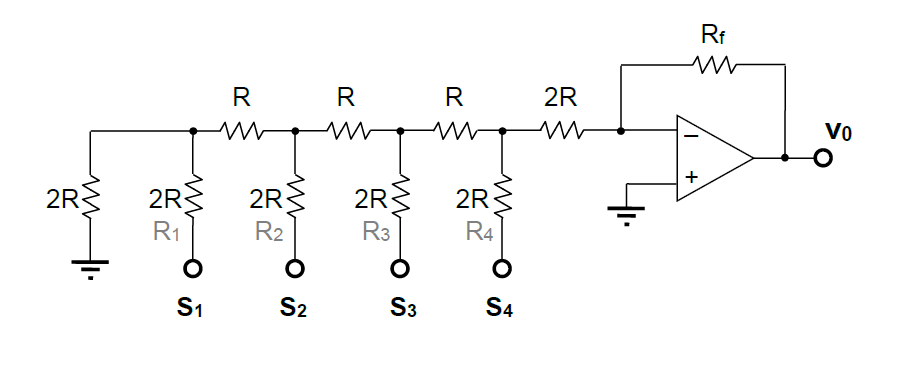
\includegraphics[angle=0,width=0.9\textwidth]{Conversor.png}
     \captionof{figure}{Circuito $DAC$ testado no laboratório.}
     \label{fig:Conversor}
     \end{center}


Podemos distinguir no circuito do conversor duas secções diferentes: um circuito em escada $R-2R$ ligado às fontes $S_1$, $S_2$, $S_3$ e $S_4$, e um circuito multiplicador inversor, sendo a sua saída, $v_o$, a saída do conversor.

Pretendemos determinar a tensão de saída do conversor em função das tensões de entrada $S_1$, $S_2$, $S_3$ e $S_4$ para 2 valores $R_f$ diferentes, $R_f=2R$ e $R_f=4R$. Recorrendo ao Princípio da Sobreposição, podemos obter $v_o$ fazendo $v_o=v_{o1}+v_{o2}+v_{o3}+v_{o4}$, em que $v_{oi}$, ($i=1,2,3,4$), corresponde à tensão de saída do conversor quando se tem apenas a fonte $S_i$ activa (isto é, quando as fontes $S_j$, $j\neq i$, são substituídas por $GND$).\\
\par

\large\underline{{\textit{\textbf{Determinação de $v_{o1}$}}}}\\
\par

Para a determinação de $v_{o1}$, substituímos as fontes $S_2$, $S_3$ e $S_4$ por \textit{ground}, obtendo-se o seguite circuito:

\begin{center}
     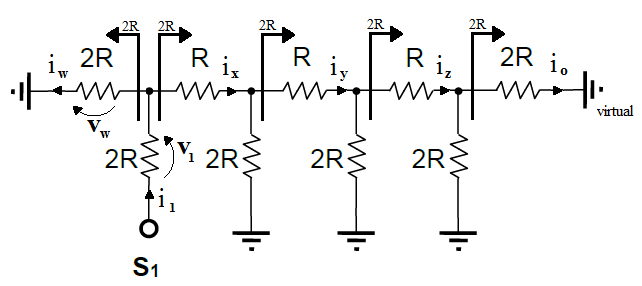
\includegraphics[angle=0,width=0.8\textwidth]{v01.png}
     \captionof{figure}{Circuito em escada do $DAC$ com as fontes $S_2$, $S_3$ e $S_4$ substituídas por $GND$, de modo a que seja possível o cálculo de  $v_{o1}$.}
     \label{fig:v01}
     \end{center}

A massa virtual evidenciada na figura \ref{fig:v01} tem origem no facto da entrada não inversora do amplificador estar ligada ao \textit{ground}, incuntindo uma tensão nula na entrada inversora (equivalente a uma massa virtual).

A resistência ``vista'' à direita de cada nó no circuito corresponde sempre a $2R$. Podemos verificar isto seguindo o seguinte raciocínio:

\begin{enumerate}

\item O ramo à direita do nó 4 (1º à direita) apresenta uma resistência $2R$ ligada à massa virtual. Portanto, a resistência ``vista'' à direita deste nó é $R'=2R$.

\item O circuito à direita do nó 3 corresponde ao equivalente de uma resistência $R$ em série com o paralelo de 2 resistências $2R$, estando o conjunto ligado à massa virtual. Portanto a resistência ``vista'' à direita do nó 3 é $R'=R+2R\parallelsum 2R=R+\frac{2R.2R}{2R+2R}=2R$.

\item A situação anterior repete-se para os restantes nós, 1 e 2.

\end{enumerate}

Para o caso do nó 1 podemos constatar que a resistência ``vista'' à sua esquerda é igualmente $R'=2R$, já que o ramo associado corresponde a uma resistência $2R$ ligada ao \textit{ground}.


Podemos obter a tensão $v_{o1}$ determinando em primeiro lugar a corrente $i_o$, e aplicando posteriormente a lei de Ohm na resistência $R_f$. Como as resistências ``vistas'' à esquerda e à direita do nó 1 são as mesmas, então a corrente $i_1$ divide-se, isto é, uma metade vai para o ramo da esquerda, e a outra metade vai para o ramo da direita $\Rightarrow i_w=i_x=\frac{i_1}{2}$. No nó 2 as resistências ``vistas'' para os ramos à direita  e inferior são as mesmas, e portanto, $i_y=\frac{i_x}{2}=\frac{i_1}{4}$. O mesmo fenómeno repete-se para os nós seguintes e ocorrem, portanto, mais duas divisões de corrente até ao último ramo da direita, sendo $i_o=\frac{i_1}{16}$.

É possível determinar $i_1$ tendo em conta que:

$$S_1=v_1+v_w=2Ri_1+2Ri_w=2Ri_1+2R\frac{i_1}{2}=3Ri_1\Leftrightarrow$$

$$\Leftrightarrow i_1=\frac{S_1}{3R}$$

Logo,
$$i_o=\frac{S_1}{3R}\frac{1}{16}$$

Aplicando a lei de Ohm na resistência $R_f$ vem que:

\begin{equation}\label{eq:v01}
v_{o1}=-R_fi_o=-\frac{R_f}{3R}\frac{S_1}{16}
\end{equation}

\large\underline{{\textit{\textbf{Determinação de $v_{o2}$}}}}\\
\par

Para este caso,  substituímos as fontes $S_1$, $S_3$ e $S_4$ por \textit{ground}, tendo-se obtido o seguinte circuito:


\begin{center}
     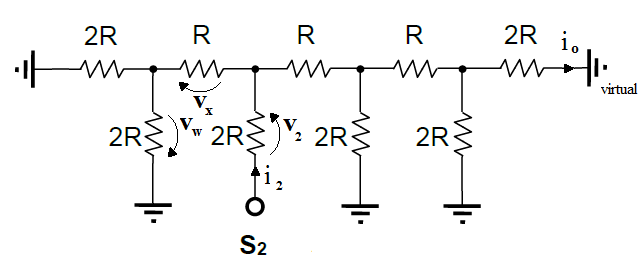
\includegraphics[angle=0,width=0.9\textwidth]{v02.png}
     \captionof{figure}{Circuito em escada do $DAC$ com as fontes $S_1$, $S_3$ e $S_4$ substituídas por $GND$.}
     \label{fig:v02}
     \end{center}
     
     
Pela análise do esquema da figura \ref{fig:v02} é possível concluir que os fenómenos de divisão sucessiva da corrente de entrada $i_2$ irão ocorrer nos vários nós, já que as resistências ``vistas'' nos ramos de chegada serão iguais.
Podemos constatar que a corrente $i_2$ irá dividir-se 3 vezes até chegar ao ramo de corrente $i_o$. Portanto,

$$i_o=\frac{i_2}{8}$$

Por outro lado, é possível determinar $i_2$ tendo em conta que:

$$S_2=v_2+v_x+v_w=2Ri_2+Ri_x+2Ri_w=2Ri_2+R\frac{i_2}{2}+2R\frac{i_2}{4}=3Ri_2\Leftrightarrow$$

$$\Leftrightarrow i_2=\frac{S_2}{3R}$$

Logo, 

$$i_o=\frac{S_2}{3R}\frac{1}{8}$$


Aplicando a lei de Ohm em $R_f$, vem que:

\begin{equation}\label{eq:v02}
v_{o2}=-\frac{R_f}{3R}\frac{S_2}{8}
\end{equation}


\large\underline{{\textit{\textbf{Determinação de $v_{o3}$}}}}\\
\par

Substituindo as fontes $S_1$, $S_2$ e $S_4$ por \textit{ground}, obteve-se o seguinte circuito:


\begin{center}
     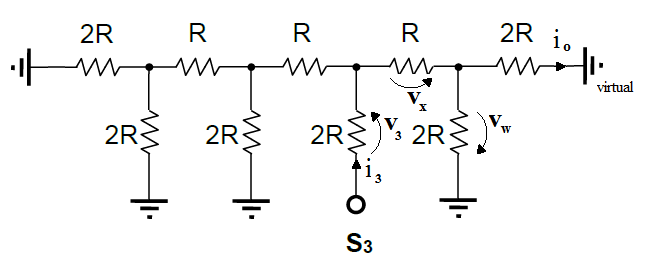
\includegraphics[angle=0,width=0.9\textwidth]{v03.png}
     \captionof{figure}{Circuito em escada do $DAC$ com as fontes $S_1$, $S_2$ e $S_4$ substituídas por $GND$.}
     \label{fig:v03}
     \end{center}

Tal como aconteceu nos casos anteriores, existem divisões sucessivas da corrente $i_3$ nos vários nós do circuito após a substituição previamente referida. Portanto, analisando o esquema, podemos constatar que:

$$i_o=\frac{i_3}{4}$$.

Tem-se que:

$$S_3=v_3+v_x+v_w=2Ri_3+R\frac{i_3}{2}+2R\frac{i_3}{4}=3Ri_3$$

$$\Leftrightarrow i_3=\frac{S_3}{3R}$$

Portanto,

$$i_o=\frac{S_3}{3R}\frac{1}{4}$$

e

\begin{equation}\label{eq:v03}
v_{o3}=-\frac{R_f}{3R}\frac{S_3}{4}
\end{equation}

\large\underline{{\textit{\textbf{Determinação de $v_{o4}$}}}}\\
\par

Substituindo as fontes $S_1$, $S_2$ e $S_3$ por \textit{ground}, obteve-se o seguinte circuito:


\begin{center}
     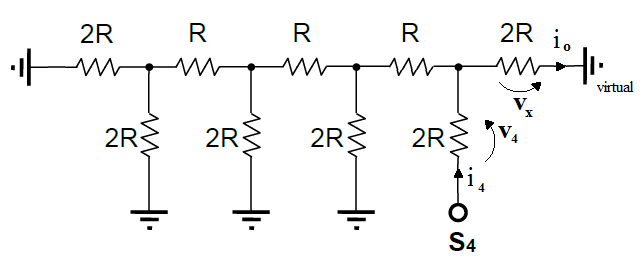
\includegraphics[angle=0,width=0.9\textwidth]{v04.png}
     \captionof{figure}{Circuito em escada do $DAC$ com as fontes $S_1$, $S_2$ e $S_3$ substituídas por $GND$.}
     \label{fig:v04}
     \end{center}

Atendendo ao fenómemo de divisão da corrente $i_4$, vem que:

$$i_o=\frac{i_4}{2}$$

sendo que,

$$S_4=v_4+v_x=2Ri_4+2Ri_o=2Ri_4+2R\frac{i_4}{2}=3Ri_4\Leftrightarrow$$

$$\Leftrightarrow i_4=\frac{S_4}{3R}$$

e portanto,

\begin{equation}\label{eq:v04}
v_{o4}=-\frac{R_f}{3R}\frac{S_4}{2}
\end{equation}


\large\underline{{\textit{\textbf{Determinação de $v_{o}$}}}}\\
\par

A partir das expressões \ref{eq:v01}, \ref{eq:v02}, \ref{eq:v03} e \ref{eq:v04} podemos calcular $v_o$, fazendo:

$$v_o=v_{o1}+v_{o2}+v_{o3}+v_{o4}=-\frac{R_f}{3R}\left(\frac{S_1}{16}+\frac{S_2}{8}+\frac{S_3}{4}+\frac{S_4}{2}\right)$$

Como $S_i=V_{Ref}b_i$, em que $b_i$ assume o valor 1, quando a fonte $S_i$ está ligada, e 0, caso contrário, tem-se que:

\begin{equation}\label{eq:v0}
v_o=-\frac{R_f}{3R}V_{Ref}\left(\frac{b_1}{16}+\frac{b_2}{8}+\frac{b_3}{4}+\frac{b_4}{2}\right)
\end{equation}


Para $R_f=2R$:

\begin{equation}\label{eq:v02R}
\boxed{v_o=-\frac{5}{3}\left(\frac{b_1}{8}+\frac{b_2}{4}+\frac{b_3}{2}+{b_4}\right)}
\end{equation}

Para $R_f=4R$:

\begin{equation}\label{eq:v04R}
\boxed{v_o=-\frac{10}{3}\left(\frac{b_1}{8}+\frac{b_2}{4}+\frac{b_3}{2}+{b_4}\right)}
\end{equation}

\section{Análise Experimental}

\subsection{Obtenção dos valores da tensão de saída, $v_o$, em função da palavra digital produzida por $S_1$, $S_2$, $S_3$ e $S_4$, com $R_f=2R$ e $R_f=4R$}

Começámos por aplicar uma onda quadrada positiva entre 0 e 5V, de frequência $f=100kHz$ no ponto $C_p$ (\textit{clock}) do conversor.

Neste circuito, a palavra digital é definida por $b_4b_3b_2b_1$, onde $b_i$ é o bit relativo ao sinal $S_i$. Isto é, um $i$ maior em $S_i$, ($i=1,2,3,4$), implica um peso maior do bit $b_i$, tal como foi possível verificar na secção anterior (ver expressão \ref{eq:v0}). Este sinal de \textit{clock} em conjunto com o contador permite-nos obter uma palavra digital, em que para o tempo do estado de $S_i$, é possível gerar os 2 estados de $S_{i+1}$, ($i=1,2,3$). O período do sinal $S_i$, corresponde a $2^i$ períodos do sinal de \textit{clock}, proporcionando num ciclo de $S_4$, a obtenção de todas as combinações possíveis de sinais para a construção das palavras digitais.

Quanto maior for o peso do sinal digital $S_i$, maior será a amplitude do sinal analógico associado. A sobreposição dos sinais irá gerar um sinal com patamares bem definidos e portanto, é possível obter $v_o$ em função da palavra $b_4b_3b_2b_1$ relacionando a amplitude de cada patamar com a sua posição relativa no tempo. É de notar que a tensão de saída $v_o(t)$ que se obtém é nao positiva, devido à operação de inversão da configuração amplificadora do conversor. Portanto, devemos de associar palavras digitais de valor superior a tensões $v_o$ absolutas maiores. \\
\par



Com os dados experimentais extraídos dos gráficos (ver figuras \ref{fig:42R} e \ref{fig:44R}) que obtivémos no osciloscópio digital, construímos a seguinte tabela de $v_o$ em função da palavra digital $b_4b_3b_2b_1$.



\begin{table}[h]
\centering
\begin{tabular}{ ||c|c| c | c | c | c | c | c || }
\hline
$b_4b_3b_1b_0$& Dec. &$S_4(V)$ & $S_3(V)$ & $S_2(V)$ & $S_1(V)$ & $v_o(V)\hspace{5pt}(R_f=2R)$ & $v_o(V)\hspace{5pt}(R_f=4R)$ \\ \hline \hline
0000&0	&0.00 & 0.00 & 0.00 & 0.00 & -0.012 $\pm$ 0.026& 0.006 $\pm$ 0.051\\ \hline
0001& 1	&0.00 & 0.00 & 0.00 & 5.00 & -0.194 $\pm$ 0.075& -0.446 $\pm$ 0.060\\ \hline
0010& 2 &	0.00 & 0.00 & 5.00 & 0.00 & -0.426 $\pm$ 0.037& -0.884 $\pm$ 0.056\\ \hline
0011&3	&0.00 & 0.00 & 5.00 & 5.00 & -0.626 $\pm$ 0.036& -1.250 $\pm$ 0.060\\ \hline
0100&4	&0.00 & 5.00 & 0.00 & 0.00 & -0.838 $\pm$ 0.047& -1.712 $\pm$ 0.001\\ \hline
0101&5	&0.00 & 5.00 & 0.00 & 5.00 & -1.047 $\pm$ 0.026& -2.0940 $\pm$ 0.060 \\ \hline
0110&6	&0.00 & 5.00 & 5.00 & 0.00 & -1.267 $\pm$ 0.034& -2.563 $\pm$ 0.047\\ \hline
0111&7	&0.00 & 5.00 & 5.00 & 5.00 & -1.478 $\pm$ 0.037& -2.977 $\pm$ 0.058\\ \hline
1000&8	&5.00 & 0.00 & 0.00 & 0.00 & -1.654 $\pm$ 0.022& -3.328 $\pm$ 0.072\\ \hline
1001&9	&5.00 & 0.00 & 0.00 & 5.00 & -1.854 $\pm$ 0.022& -3.749 $\pm$ 0.053\\ \hline
1010&10	&5.00 & 0.00 & 5.00 & 0.00 & -2.081 $\pm$ 0.043& -4.184 $\pm$ 0.072\\ \hline
1011&11	&5.00 & 0.00 & 5.00 & 5.00 & -2.278 $\pm$ 0.001& -4.566 $\pm$ 0.040\\ \hline
1100&12	&5.00 & 5.00 & 0.00 & 0.00 & -2.501 $\pm$ 0.022& -5.029 $\pm$ 0.060\\ \hline
1101&13	&5.00 & 5.00 & 0.00 & 5.00 & -2.697 $\pm$ 0.023& -5.411 $\pm$ 0.080 \\ \hline
1110&14	&5.00 & 5.00 & 5.00 & 0.00 & -2.917 $\pm$ 0.036& -5.864 $\pm$ 0.051\\ \hline
1111&15	&5.00 & 5.00 & 5.00 & 5.00 & -3.122 $\pm$ 0.001& -6.255 $\pm$ 0.040 \\ \hline
\end{tabular}


\caption{Valores experimentais da tensão $v_o(V)$ em função da palavra $b_4b_3b_2b_1$ para $R_f=2R$ e $R_f=4R$. Os erros $e_{v_o}(V)$ correspondem aos desvios máximos em relação à média.\label{tab:4}}

\end{table}

É de notar que o erro $e_{v_o}$ para $b_4b_3b_2b_1=0000$ é superior ao valor $v_o$ associado, e portanto, $v_o$ neste caso, tem origem no ruído da montagem experimental.

\subsection{Obtenção das formas de onda dos gráficos $v_o(t)$ e $v_{Clk}(t)$ para $R_f=2R$ e $R_f=4R$ a partir do osciloscópio digital}

Obtivémos a partir do osciloscópio digital os seguinte gráficos dos sinais de saída do conversor, $v_o(t)$, e de \textit{clock}, $v_{Clk}(t)$, para $R_f=2R$ e $R_f=4R$:

\begin{center}
     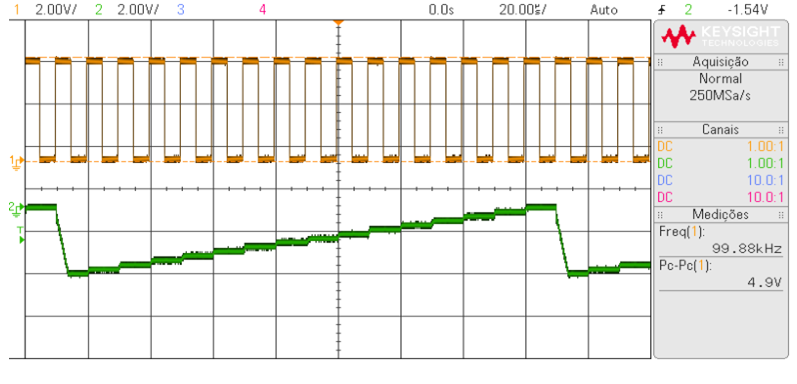
\includegraphics[angle=0,width=0.9\textwidth]{42R.png}
     \captionof{figure}{Gráficos $v_o(t)$ (a verde) e $v_{Clk}(t)$ (a laranja) para $R_f=2R$ obtidos pelo osciloscópio digital via \textit{Microsoft Excel}.}
     \label{fig:42R}
     \end{center}
     
\begin{center}
     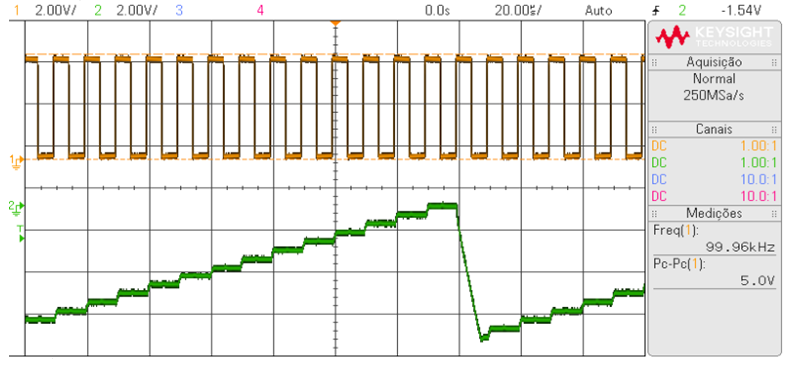
\includegraphics[angle=0,width=0.9\textwidth]{44R.png}
     \captionof{figure}{Gráficos $v_o(t)$ (a verde) e $v_{Clk}(t)$ (a laranja) para $R_f=4R$ obtidos pelo osciloscópio digital via \textit{Microsoft Excel}.}
     \label{fig:44R}
     \end{center}


\subsection{Variação da tensão de saída do conversor observada entre dois níveis consecutivos, para os dois valores diferentes de $R_f$ } 

Podemos constatar pela análise dos gráficos das figuras \ref{fig:42R} e \ref{fig:44R} que as variações da tensão $v_o$ entre níveis consecutivos são praticamente uniformes entre si, sendo que se verificou para $R_f=4R$ um maior passo incremental de tensão que para $R_f=2R$. Este facto pode ser explicado pela expressão \ref{eq:v0}, já que $v_o\propto R_f$.

De forma a analisarmos este comportamento quantitativamente, construímos a seguinte tabela de variações $v_o$ entre níveis consecutivos, para $R_f=2R$ e $R_f=4R$:

\begin{table}[h]
\begin{center}
\begin{tabular}{ || c | c | c | c || }
\hline
	$b_4b_3b_2b_1$ & Dec. & $|\Delta v_o|(V)$ $(Rf=2R)$ & $|\Delta v_o|(V)$ $(Rf=4R)$ \\ \hline \hline
	0000 & 0 & --- & --- \\ \hline
	0001 & 1 & 0.181 $\pm$ 0.078 & 0.451 $\pm$ 0.079 \\ \hline
	0010 & 2 & 0.232 $\pm$ 0.083& 0.438 $\pm$ 0.082 \\ \hline
	0011 & 3 & 0.201 $\pm$ 0.052& 0.365 $\pm$ 0.082 \\ \hline
	0100 & 4 & 0.211 $\pm$ 0.059 & 0.462 $\pm$ 0.060\\ \hline
	0101 & 5 & 0.208 $\pm$ 0.053 & 0.381 $\pm$ 0.060 \\ \hline
	0110 & 6 & 0.219 $\pm$ 0.042 & 0.469 $\pm$ 0.076 \\ \hline
	0111 & 7 & 0.211 $\pm$ 0.050 & 0.413 $\pm$ 0.074 \\ \hline
	1000 & 8 & 0.175 $\pm$ 0.042& 0.351 $\pm$ 0.093 \\ \hline
	1001 & 9 & 0.200 $\pm$ 0.031 & 0.420 $\pm$ 0.090 \\ \hline
	1010 & 10 & 0.226 $\pm$ 0.048 & 0.435 $\pm$ 0.113 \\ \hline
	1011 & 11 & 0.197 $\pm$ 0.044 & 0.381 $\pm$ 0.108 \\ \hline
	1100 & 12 & 0.222 $\pm$ 0.021 & 0.462 $\pm$ 0.072\\ \hline
	1101 & 13 & 0.196 $\pm$ 0.032 & 0.381 $\pm$ 0.100 \\ \hline
	1110 & 14 & 0.220 $\pm$ 0.043 & 0.453 $\pm$ 0.095 \\ \hline
	1111 & 15 & 0.205 $\pm$ 0.036 & 0.391 $\pm$ 0.065 \\ \hline
\end{tabular}

\caption{Valores experimentais da variação de tensão, $|\Delta v_o|(V)$, entre palavras consecutivas $b_4b_3b_2b_1$ para $R_f=2R$ e $R_f=4R$.\label{tab:4.1}}
\end{center}
\end{table}

%%%%%%%%%%%%%%%%%este vspace poderá originar problemas. adicionei-o porque o texto ficava antes da tabela%%%%%%%%%%%%%%%%%%%%%%%%%%%%%%%%%%%%%%%%%%%%%%%%%%%%%%
\vspace{110pt}
%%%%%%%%%%%%%%%%%%%%%%%%%%%%%%%%%%%%%%%%%%%%%%%%%%%%%%%%%%%%%%%%%%%%%%%%%%%%%%%%%%%%%%%%%%%%%%%%%%%%%%%%%%%%%%%%%%%%%%%%%%%%%%%%%%%%%%%%%%%%%%%%%%%%%%%%%%%%%%
Antes de determinarmos o valor esperado para o passo entre patamares consecutivos, podemos em primeiro lugar verificar se os incrementos são realmente uniformes.
Com os dados da tabela \ref{tab:4.1} realizámos ajustes gráficos, recorrendo à função-base $y=ax+b$, de $|\Delta v_o| (V)$ vs \textit{Palavra decimal} para $R_f=2R$ (figura \ref{fig:2R}) e $R_f=4R$ (figura \ref{fig:4R}).


\begin{center}
     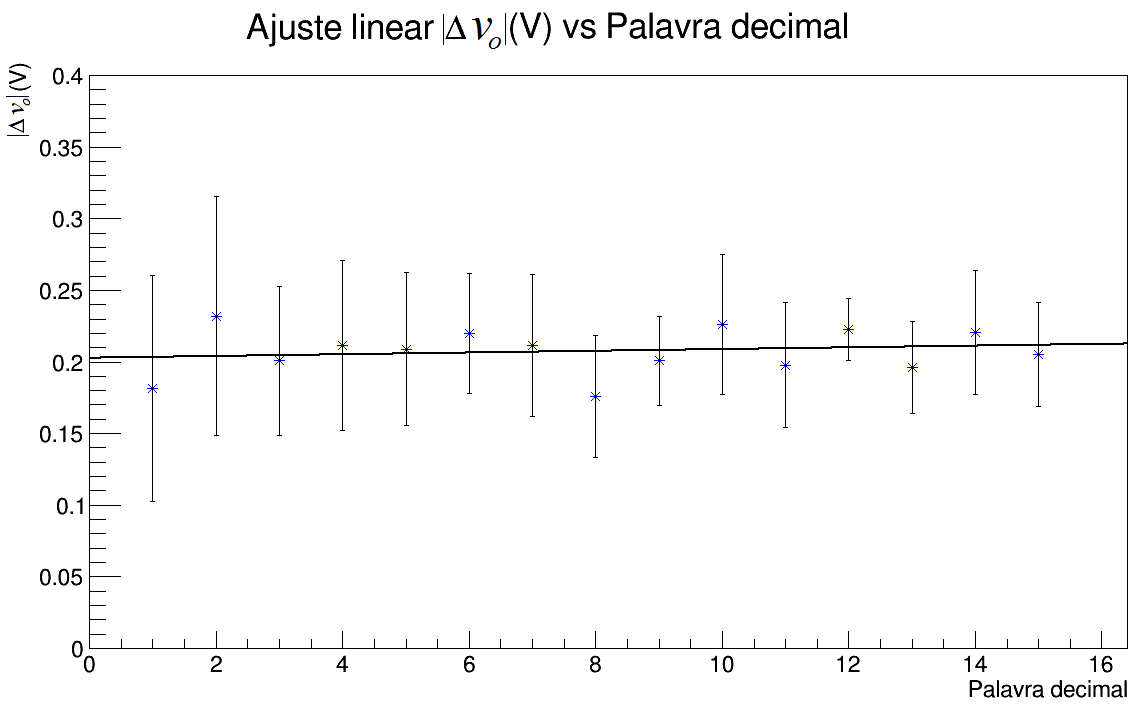
\includegraphics[angle=0,width=0.9\textwidth]{2R.png}
     \captionof{figure}{Ajuste, pelo método dos mínimos quadrados, de $|\Delta v_o| (V)$ vs \textit{Palavra decimal} para $R_f=2R$, via \textit{ROOT}. }
     \label{fig:2R}
     \end{center}



     
\begin{center}
     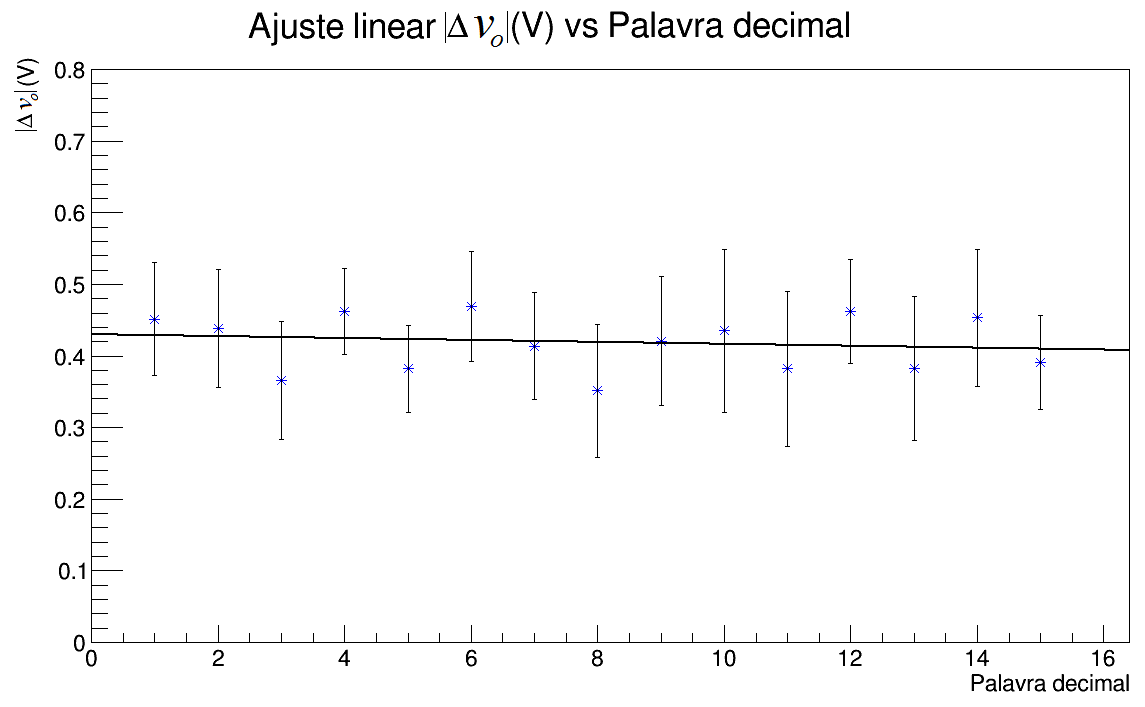
\includegraphics[angle=0,width=0.9\textwidth]{4R.png}
     \captionof{figure}{Ajuste, pelo método dos mínimos quadrados, de $|\Delta v_o| (V)$ vs \textit{Palavra decimal} para $R_f=4R$, via \textit{ROOT}.}
     \label{fig:4R}
     \end{center}


Obtivémos do ajuste linear $|\Delta v_o| (V)$ vs \textit{Palavra decimal} para $R_f=2R$ (figura \ref{fig:2R}), os seguintes resultados:

\begin{table}[h]
\begin{center}
\begin{tabular}{ || c | c | c || }
\hline
$a(V)$ & $b(V)$ &  $X^2_{ndf}$\\ \hline \hline
$\left(6.043 \pm 28.763 \right)\times 10^{-4}$ & $0.203 \pm 0.030$ &0.137\\ \hline

\end{tabular}

\caption{Resultados do ajuste $|\Delta v_o| (V)$ vs \textit{Palavra decimal}, para $R_f=2R$.\label{tab:res2R}}
\end{center}
\end{table}

Podemos constatar que o declive da reta de ajuste, $a$, corresponde a um valor aproximadamente nulo, sendo que o próprio erro o suplanta. Portanto a reta de ajuste será uma boa aproximação de uma reta constante $y=b$.  Sendo assim, o valor de $b$ dará uma boa estimativa do valor de $|\Delta v_{o_{exp}}|$ para o caso de $R_f=2R$. \\
\par
Obtivémos para o caso do ajuste linear $|\Delta v_o| (V)$ vs \textit{Palavra decimal} com $R_f=4R$ (figura \ref{fig:4R}), os seguintes resultados:

\begin{table}[h]
\begin{center}
\begin{tabular}{ || c | c | c || }
\hline
$a(V)$ & $b(V)$ &  $X^2_{ndf}$\\ \hline \hline
$-0.001 \pm 0.005$ & $0.429 \pm 0.040$ &0.258\\ \hline

\end{tabular}

\caption{Resultados do ajuste $|\Delta v_o| (V)$ vs \textit{Palavra decimal}, para $R_f=4R$.\label{tab:res2R}}
\end{center}
\end{table}

Tal como verificámos para $R_f=2R$, o declive da reta de ajuste $a$, corresponde a um valor aproximadamente nulo em que o próprio erro o suplanta. Portanto a reta de ajuste $|\Delta v_o| (V)$ vs \textit{Palavra decimal} para $R_f=4R$ será igualmente uma boa aproximação de uma reta constante $y=b$. O valor de $b$ dará uma ideia do valor de $|\Delta v_{o_{exp}}|$ para o caso de $R_f=4R$.\\
\par
Para a determinação do valor esperado para o passo entre patamares consecutivos, é necessário obter o declive da reta $y=a\times x+b$ que melhor se ajusta aos pontos $(Palavra$ $decimal,v_o)$.

Com os dados da tabela \ref{tab:4} realizámos ajustes lineares, de $|v_o| (V)$ vs \textit{Palavra decimal} para $R_f=2R$ (figura \ref{fig:2Rpasso}) e $R_f=4R$ (figura \ref{fig:4Rpasso}).

\begin{center}
     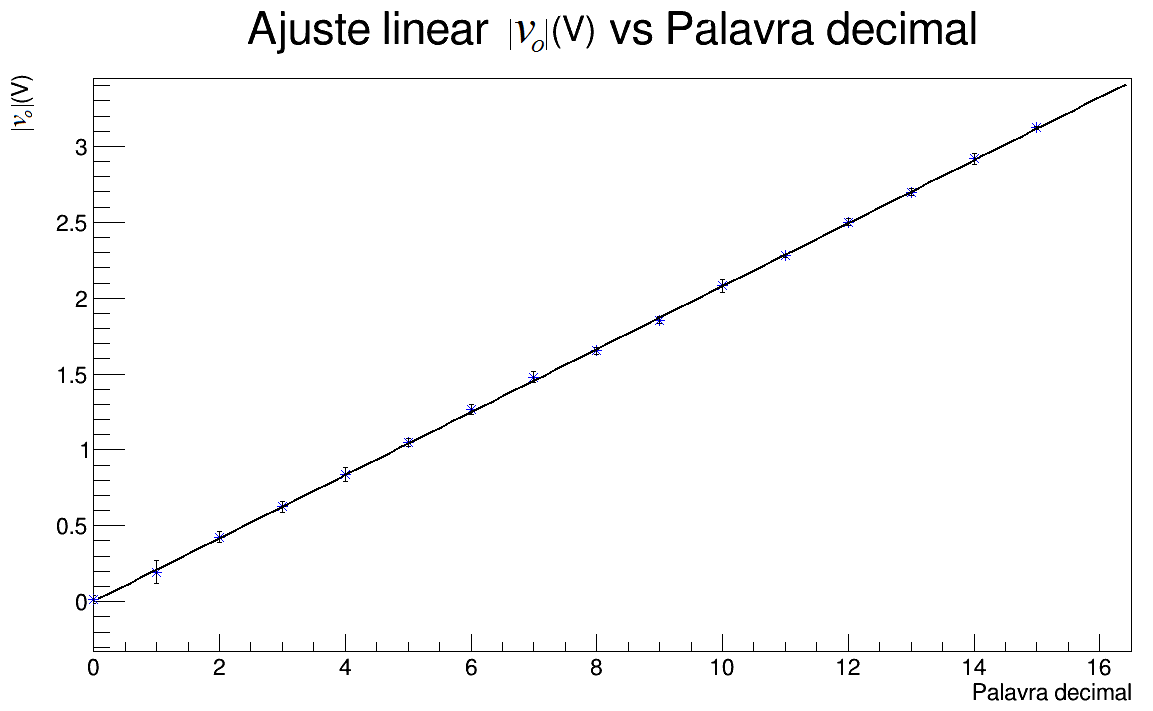
\includegraphics[angle=0,width=0.9\textwidth]{2Rpasso.png}
     \captionof{figure}{Ajuste, pelo método dos mínimos quadrados, de $|v_o| (V)$ vs \textit{Palavra decimal} para $R_f=2R$, via \textit{ROOT}. }
     \label{fig:2Rpasso}
     \end{center}



     
\begin{center}
     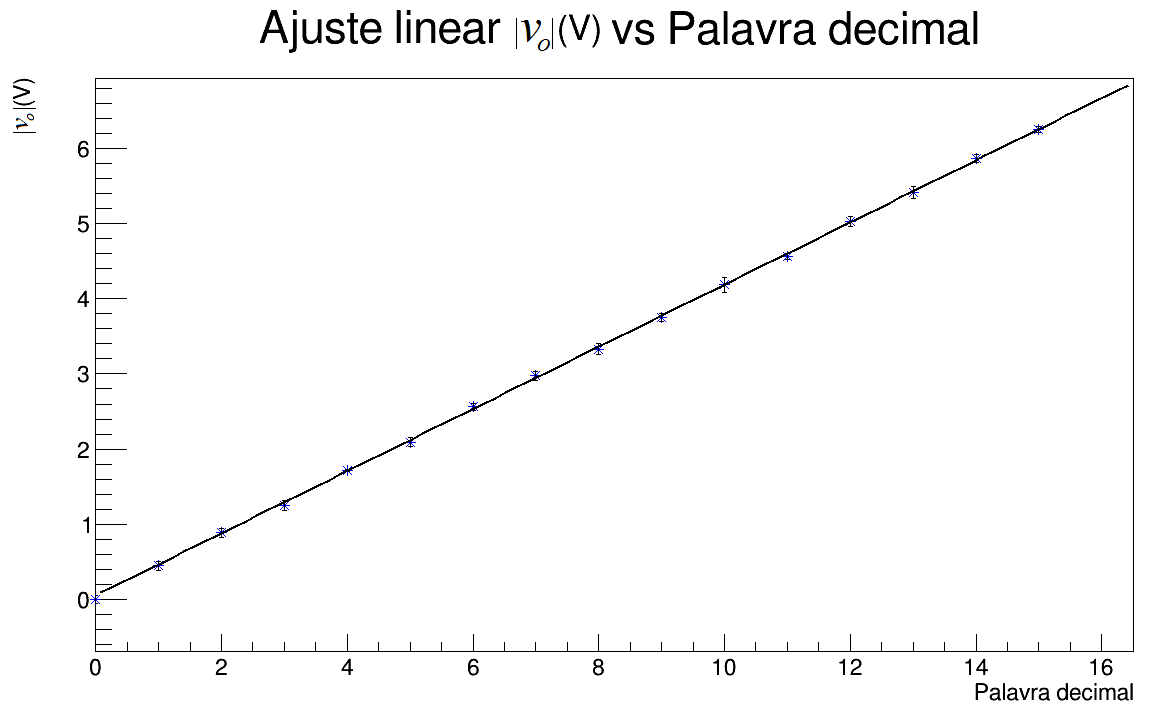
\includegraphics[angle=0,width=0.9\textwidth]{4Rpasso.png}
     \captionof{figure}{Ajuste, pelo método dos mínimos quadrados, de $|v_o| (V)$ vs \textit{Palavra decimal} para $R_f=4R$, via \textit{ROOT}.}
     \label{fig:4Rpasso}
     \end{center}


Obtivémos para o ajuste linear $|v_o| (V)$ vs \textit{Palavra decimal} para o caso $R_f=2R$ os seguintes resultados:

\begin{table}[h]
\begin{center}
\begin{tabular}{ || c | c | c || }
\hline
$a(V)$ & $b(V)$ &  $X^2_{ndf}$\\ \hline \hline
$0.208 \pm 0.001$ & $0.003 \pm 0.015$ &0.209\\ \hline

\end{tabular}

\caption{Resultados do ajuste $|v_o| (V)$ vs \textit{Palavra decimal}, para $R_f=2R$.\label{tab:res2Rpasso}}
\end{center}
\end{table}

O valor do parâmetro $a=0.208 \pm 0.001 V$ indica-nos que a variação da tensão $v_o$ entre níveis consecutivos (passo) para $R_f=2R$ foi aproximadamente:

\begin{equation}\label{eq:v02Rexp}
\boxed{|\Delta v_{o_{exp}}|=0.208 \pm 0.001V}
\end{equation}


Obtivémos para o ajuste linear $|v_o| (V)$ vs \textit{Palavra decimal} para o caso $R_f=4R$ que:

\begin{table}[h]
\begin{center}
\begin{tabular}{ || c | c | c || }
\hline
$a(V)$ & $b(V)$ &  $X^2_{ndf}$\\ \hline \hline
$0.414 \pm 0.002$ & $0.052 \pm 0.016$ &0.323\\ \hline

\end{tabular}

\caption{Resultados do ajuste $|v_o| (V)$ vs \textit{Palavra decimal}, para $R_f=4R$.\label{tab:res4Rpasso}}
\end{center}
\end{table}


E portanto, o valor do parâmetro $a=0.414 \pm 0.002 V$ indica-nos que o passo entre níveis consecutivos, para $R_f=4R$, foi aproximadamente:

\begin{equation}\label{eq:v04Rexp}
\boxed{|\Delta |v_{o_{exp}}|=0.414 \pm 0.002V}
\end{equation}

\vspace{15pt}
\large\underline{{\textit{\textbf{Comentário e comparação de resultados}}}}\\
\par

Podemos determinar o valor teórico para o passo entre níveis consecutivos para $R_f=2R$ e $R_f=4R$, tendo em conta as expressões \ref{eq:v02R} e \ref{eq:v04R} respectivamente. O passo incremental corresponderá ao valor de $v_o$ associado à palavra $b_4b_3b_2b_1=0001$, isto é, quando $b_4=0$, $b_3=0$, $b_2=0$ e $b_1=0$.
Recorrendo a \ref{eq:v02R} e \ref{eq:v04R} e associando o índice ``1'' a $R_f=2R$ e ``2'' a $R_f=4R$, tem-se que:


\begin{equation}\label{eq:v02Rpassoteo}
\boxed{|\Delta v_{o1_{teo}}|=\frac{5}{24}\approx0.208(33)\hspace{10pt}\Rightarrow \sigma_{exat.}\approx 0}
\end{equation}

\begin{equation}\label{eq:v04Rpassoteo}
\boxed{|\Delta v_{o2_{teo}}|=\frac{5}{12}\approx0.416(66)\hspace{38pt}\Rightarrow \sigma_{exat.}=0.48\%}
\end{equation}

em que $\sigma_{exat.}$ corresponde ao desvio à exatidão dos valores $|\Delta v_o|$ experimentais expressos em \ref{eq:v02Rexp} e \ref{eq:v04Rexp} respectivamente. Como os valores  $\sigma_{exat.}$ são aproximadamente nulos é correcto dizer que os resultados experimentais de $|\Delta v_o|$ foram os teoricamente previstos.\\
\par
Podemos ainda dizer por \ref{eq:v02Rexp} e \ref{eq:v04Rexp} que a variação da tensão $v_o$ entre níveis consecutivos para $R_f=4R$ foi praticamente 2 vezes superior à correspondente a $R_f=2R$. Tem-se que:

\begin{equation}\label{eq:rel}
\boxed{\left(\frac{|\Delta v_{o_2}|}{|\Delta v_{o_{1}}|}\right)_{exp}=1.99\pm 0.002,\hspace{15pt}\sigma_{exat.}=0.5\%}
\end{equation}

O valor teórico  $\left(\frac{|\Delta v_{o_2}|}{|\Delta v_{o_{1}}|}\right)_{teo}=2$ obtém-se trivialmente pela a expressão \ref{eq:v0} já que $R_{f2}=4R=2R_{f1}$. Podemos assim notar que $\left(\frac{|\Delta v_{o_2}|}{|\Delta v_{o_{1}}|}\right)_{exp}$ e $\left(\frac{|\Delta v_{o_2}|}{|\Delta v_{o_{1}}|}\right)_{teo}$ são praticamente coincidentes.



Relativamente às discrepâncias individuais dos valores dos patamares $v_o$ face aos valores teóricos, podemos construir a seguinte tabela:

\begin{table}[h]
\centering
\begin{tabular}{ || c| c || c | c | c|| c | c | c || }
\hline
	$b_4b_3b_2b_1$ & Dec. & $v_{o1_{exp}}(V)$ & $v_{o1_{teo}}(V)$& $\sigma_{exat.1}(\%)$ & $v_{o2_{exp}}(V)$ & $v_{o2_{teo}}(V)$ & $\sigma_{exat.2}(\%)$\\ \hline\hline
	0000 & 0 & -0 & 0 & 0 & 0 & 0 & 0 \\ \hline
	0001 & 1 & -0.193 & -0.208 & 7.092 & -0.445 & -0.416 & 6.975 \\ \hline
	0010 & 2 & -0.425 & -0.416 & 2.160& -0.883& -0.833 & 6.070\\ \hline
	0011 & 3 & -0.626 & -0.625 & 0.219 & -1.249& -1.250 & 2.013\\ \hline
	0100 & 4 & -0.837 & -0.833 & 0.527 & -1.712& -1.666 & 2.724\\ \hline
	0101 & 5 & -1.046 & -1.041 & 0.478 & -2.093& -2.083 & 0.511 \\ \hline
	0110 & 6 & -1.266 & -1.250 & 1.323& -2.562 & -2.500 & 2.519\\ \hline
	0111 & 7 & -1.477 & -1.458 & 1.341 & -2.976 & -2.916 & 2.054 \\ \hline
	1000 & 8 & -1.653 & -1.666 & 0.783 & -3.328 & -3.333 & 0.156 \\ \hline
	1001 & 9 & -1.854 & -1.875 & 1.102 & -3.748 & -3.750 & 2.905\\ \hline
	1010 & 10 & -2.080 & -2.083 & 0.130 & -4.184 & -4.166 & 0.426\\ \hline
	1011 & 11 & -2.278 & -2.291 & 0.584 & -4.566 & -4.583 & 0.371\\ \hline
	1100 & 12 & -2.500 & -2.500 & 0.036 & -5.028 & -5.000 & 0.573 \\ \hline
	1101 & 13 & -2.697 & -2.708 & 0.417 & -5.410 & -5.416 & 0.113\\ \hline
	1110 & 14 & -2.917 & -2.916 & 0.027& -5.863 & -5.833 & 0.521 \\ \hline
	1111 & 15 & -3.122 & -3.125 & 0.080 & -6.254 & -6.250 & 0.006 \\ \hline
\end{tabular}

\caption{Valores experimentais e teóricos de $v_o(V)$ em função da palavra $b_4b_3b_2b_1$, com os desvios à exactidão, $\sigma_{exat.}$, associados.\label{tab:comp}}
\end{table}

 É importante referir que considerámos na tabela \ref{tab:comp}, $v_{o1_{exp}}=0$ e $v_{o2_{exp}}=0$ para a palavra $b_4b_3b_2b_1=0000$, pois para este caso, obtiveram-se erros experimentais $e_{v_o}$ superiores ao próprio valor $v_o$, em que $v_o\approx0$.
 
Analisando os desvios à exactidão, $\sigma_{exat.}$, evidenciados na tabela anterior, podemos concluir que os valores de $v_o$ que obtivémos experimentalmente foram bastante próximos dos teóricos, já que que o valor máximo dos desvios obtidos foi $\sigma_{{exat.}_{máx}}=7.092\%$. Isto revela que a experiência executada no laboratório  pode ser explicada pela fundamentação teórica que anteriormente formulámos.

\chapter{Influência das resistências de entrada}

\section{Análise Teórica}

\subsection{Determinação da influência da variação das resistências $R_1$ a $R_4$, variando uma de cada vez}

Nesta secção iremos fazer uma análise semelhante ao que foi feito anteriormente, mas agora alterando o valor de uma das resistências $R_i$ $(i=1,2,3,4)$ de cada vez. Desta forma, em vez de todas as resistências tomarem o valor $2R$, admitimos que a resistência alterada tem o valor $R_i$, e as restantes o valor $2R$, como anteriormente.

Começamos então por determinar o valor da tensão $v_o$, para um qualquer valor de $R_1$.\\

\par

\large\underline{\textit{\textbf{$R_1$ - Determinação de $v_{o1}$}}}\\
\par

Para determinar o valor de $v_o1$, iremos substituir as fontes $S_2$, $S_3$ e $S_4$ por \textit{ground}, tal como fizemos na análise da secção anterior, obtendo-se o gráfico da figura \ref{fig:v01_alt}:

\begin{center}
     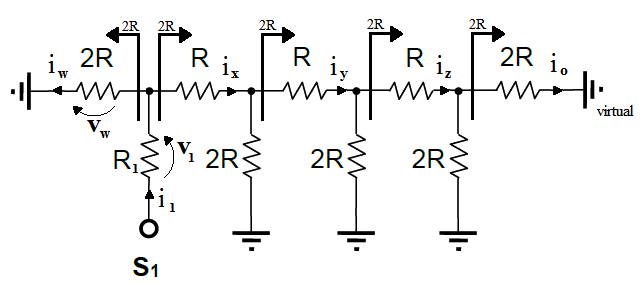
\includegraphics[angle=0,width=0.9\textwidth]{v01_alt.png}
     \captionof{figure}{Circuito em escada do $DAC$ com as fontes $S_2$, $S_3$ e $S_4$ substituídas por $GND$.}
     \label{fig:v01_alt}
     \end{center}

Desta forma, a corrente $i_o$ vai ser igual à calculada na secção anterior, tendo o valor $i_o=\frac{i_1}{16}$.

Agora para determinar o valor de $i_1$ temos:

$$S_1=v_1+v_w=R_1 i_1+2R i_w=R_1 i_1 +2R \frac{i_1}{2}=\left(R_1+R\right)i_1\Leftrightarrow $$

$$\Leftrightarrow i_1=\frac{S_1}{R_1+R}$$

Logo,

$$i_o=\frac{S_1}{R_1+R}\frac{1}{16}$$

Aplicando agora a lei de Ohm em $R_f$, obtemos:

\begin{equation}\label{eq:v01_1}
v_{01}=-R_fi_o=-\frac{R_f}{R_1+R}\frac{S_1}{16}
\end{equation}\\

\par

\large\underline{\textit{\textbf{$R_1$ - Determinação de $v_{o2}$}}}\\
\par

Neste ponto, substituímos as fontes $S_1$,  $S_3$ e $S_4$ por \textit{ground}, obtendo o circuito da \ref{fig:v02_alt}:

\begin{center}
     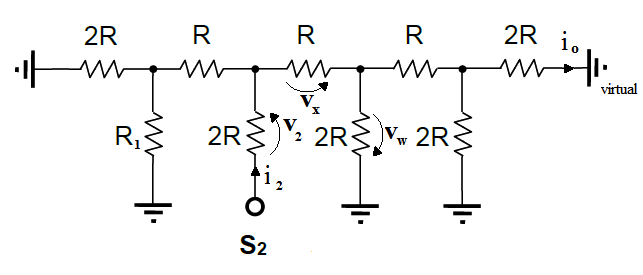
\includegraphics[angle=0,width=0.9\textwidth]{v02_alt.png}
     \captionof{figure}{Circuito em escada do $DAC$ com as fontes $S_1$, $S_3$ e $S_4$ substituídas por $GND$.}
     \label{fig:v02_alt}
     \end{center}

Fazendo a análise das resistências ``vistas'' à direita e à esquerda do nó 2, verificamos que a resistência à direita continua a ser $2R$, como na secção anterior, mas a resistência à esquerda vai ser diferente, a que damos o nome de $R_1'$:

$$R_1'=R+\left(2R\parallelsum R_1\right)=R+\frac{2R.R_1}{2R+R_1}$$

\begin{center}
     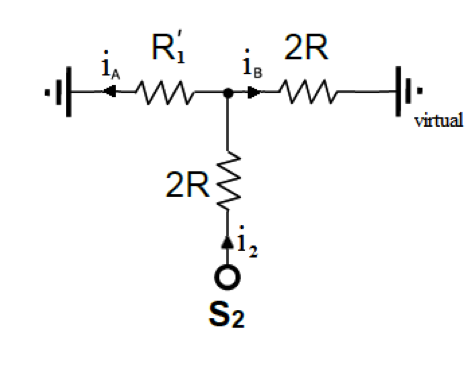
\includegraphics[angle=0,width=0.5\textwidth]{div_2.png}
     \captionof{figure}{Divisor de corrente no nó 2.}
     \label{fig:div_2}
     \end{center}

Fazendo agora um divisor de corrente no nó 2, como apresentado na figura \ref{fig:div_2}, verificamos que a corrente para a esquerda vai ser $i_A=\frac{v_2'}{R_1'}$ e a corrente para a direita vai ser $i_B=\frac{v_2'}{2R}$, sendo $v_2'$ a tensão no nó 2:
%%%%%%%%%%% Inserir figuras do divisor de corrente!!!! %%%%%%%%%%%

$$v_2'=i_2\left(R_1'\parallelsum 2R\right)=i_2\frac{R_1'.2R}{R_1'+2R}$$

Obtemos assim a expressão para a corrente à direita do nó 2:

$$\Rightarrow i_B=i_2\frac{R_1'}{R_1'+2R}$$

Neste caso a corrente $i_B$ irá ser dividida duas vezes até chegar a $i_o$, pelo que esta corrente é dada por:

$$i_o=\frac{i_B}{4}=\frac{1}{4}\frac{R_1'}{R_1'+2R}i_2$$

Agora para determinar o valor de $i_2$ temos:

$$S_2=v_2+v_x+v_w=2Ri_2+Ri_B+2R\frac{i_B}{2}=2R\left(i_2+i_B\right)=2R\left(1+\frac{R_1'}{R_1'+2R}\right) i_2$$

$$\Rightarrow i_2=\frac{S_2}{2R\left(1+\frac{R_1'}{R_1'+2R}\right)}$$

Aplicando de novo a lei de Ohm em $R_f$, obtemos:

$$v_{02}=-R_f.i_o=-\frac{1}{4}.\frac{R_fR_1'}{R_1'+2R}.\frac{S_2}{2R\left(1+\frac{R_1'}{R_1'+2R}\right)}$$

\begin{equation}\label{eq:v02_1}
\Rightarrow v_{o2}=-\frac{R_f}{R\left(1+\frac{R}{R_1'}\right)}.\frac{S_2}{16}
\end{equation}\\

\par

\large\underline{\textit{\textbf{$R_1$ - Determinação de $v_{o3}$}}}\\
\par

Substituindo as fontes $S_1$, $S_2$ e $S_4$ por \textit{ground}, obtivemos o circuito da \ref{fig:v03_alt}:

\begin{center}
     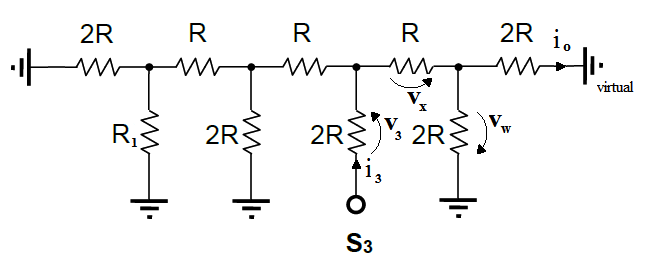
\includegraphics[angle=0,width=0.9\textwidth]{v03_alt.png}
     \captionof{figure}{Circuito em escada do $DAC$ com as fontes $S_1$, $S_2$ e $S_4$ substituídas por $GND$.}
     \label{fig:v03_alt}
     \end{center}
     
Fazendo agora a análise das resistências ``vistas'' à direita e à esquerda do nó 3, verificamos que a resistência equivalente à direita continua a ter o valor $2R$, e a resistência equivalente à esquerda, a que damos o nome de $R_1''$ tem o seguinte valor:

$$R_1''=R+\left(2R\parallelsum R_1'\right)=R+\frac{2R.R_1'}{2R+R_1'}$$

\begin{center}
     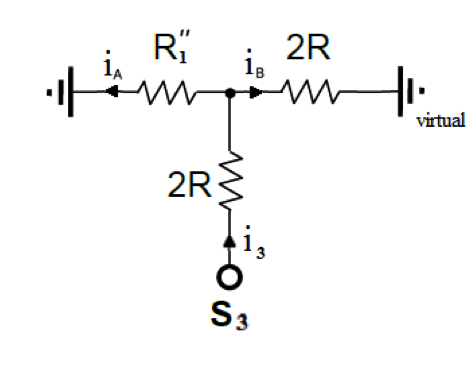
\includegraphics[angle=0,width=0.5\textwidth]{div_3.png}
     \captionof{figure}{Divisor de corrente no nó 3.}
     \label{fig:div_3}
     \end{center}

Ao fazer de novo um divisor de corrente, agora no nó 3, como representado na figura \ref{fig:div_3}, obtemos a corrente que vai para a esquerda do nó, $i_A=\frac{v_3'}{R_1''}$, e a que vai para a direita, $i_B=\frac{v_3'}{2R}$. A tensão no nó 3, $v_3'$ obtém-se fazendo o paralelo das resistências equivalentes:

$$v_3'=i_3\left(R_1''\parallelsum 2R\right)=i_3\frac{R_1''.2R}{R_1''+2R}$$

Vem assim o valor da corrente à direita do nó 3:

$$i_B=i_3\frac{R_1''}{R_1''+2R}$$

A corrente $i_B$ vai agora ser dividida apenas uma vez, até à corrente $i_o$, que é dada por:

$$i_o=\frac{i_B}{2}=\frac{1}{2}.\frac{R_1''}{R_1''+2R}i_3$$

Para determinar o valor de $i_3$ vem:

$$S_3=v_3+v_x+v_w=2Ri_3+Ri_B+2R\frac{i_B}{2}=2R\left(i_3+i_B\right)=2R\left(1+\frac{R_1''}{R_1''+2R}\right)i_3$$

$$\Rightarrow i_3=\frac{S_3}{2R\left(1+\frac{R_1''}{R_1''+2R}\right)}$$

Aplicando a lei de Ohm em $R_f$ obtemos então:

$$v_{o3}=-R_f.i_o=-\frac{1}{2}.\frac{R_fR_1''}{R_1''+2R}.\frac{S_3}{2R\left(1+\frac{R_1''}{R_1''+2R}\right)}$$

\begin{equation}\label{eq:v03_1}
\Rightarrow v_{o3}=-\frac{R_f}{R\left(1+\frac{R}{R_1''}\right)}\frac{S_3}{8}
\end{equation}\\

\par

\large\underline{\textit{\textbf{$R_1$ - Determinação de $v_{o4}$}}}\\
\par

De forma semelhante ao que fizemos nos casos anteriores, substituímos as fontes $S_1$,  $S_2$ e $S_3$ por \textit{ground}, obtendo o circuito da \ref{fig:v04_alt}:

\begin{center}
     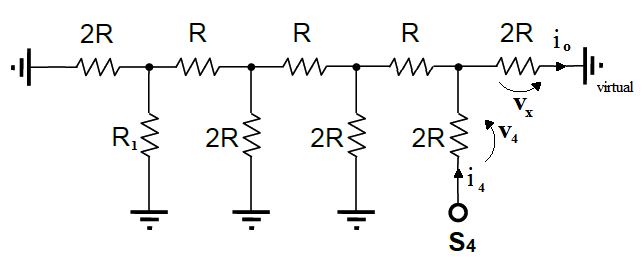
\includegraphics[angle=0,width=0.9\textwidth]{v04_alt.png}
     \captionof{figure}{Circuito em escada do $DAC$ com as fontes $S_1$, $S_2$ e $S_3$ substituídas por $GND$.}
     \label{fig:v04_alt}
     \end{center}

Fazendo a mesma análise das resistências equivalentes, desta vez para o nó 4, obtemos à direita o valor $2R$, e à esquerda $R_2'''$:

$$R_1'''=R+\left(2R\parallelsum R_1''\right)=R+\frac{2R.R_1''}{2R+R_1''}$$

\begin{center}
     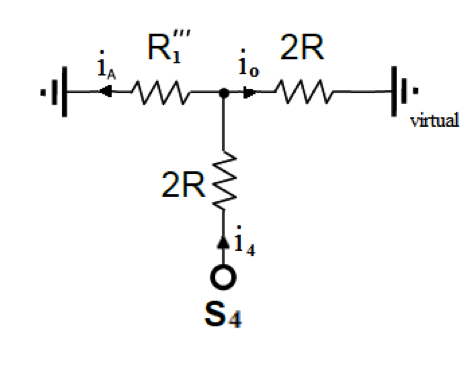
\includegraphics[angle=0,width=0.5\textwidth]{div_4.png}
     \captionof{figure}{Divisor de corrente no nó 4.}
     \label{fig:div_4}
     \end{center}

Fazendo o divisor de corrente a partir do nó 4, como representado na figura \ref{fig:div_4}, obtemos o valor da corrente que vai para a esquerda, $i_A=\frac{v_4'}{R_1'''}$, e da corrente que vai para a direita, $i_o=\frac{v_4'}{2R}$, sendo a tensão no nó 4, $v_4'$:

$$v_4'=i_4\left(R_1'''\parallelsum 2R\right)=\frac{R_1'''.2R}{R_1'''+2R}i_4$$

Ficando assim:

$$i_o=\frac{R_1'''}{R_1'''+2R}i_4$$

Agora para determinar o valor de $i_4$:

$$S_4=v_4+v_x=2R.i_4+2R.i_o=2R\left(1+\frac{R_1'''}{R_1'''+2R}\right)i_4$$

$$\Rightarrow i_4=\frac{S_4}{2R\left(1+\frac{R_1'''}{R_1'''+2R}\right)}$$

Aplicando agora a lei de Ohm em $R_f$ obtemos então:

$$v_{04}=-R_f.i_o=-\frac{R_fR_1'''}{R_1'''+2R}.\frac{S_4}{2R\left(1+\frac{R_1'''}{R_1'''+2R}\right)}$$

\begin{equation}\label{eq:v04_1}
\Rightarrow v_{o4}=-\frac{R_f}{R\left(1+\frac{R}{R_1'''}\right)}\frac{S_4}{4}
\end{equation}\\

\par

\large\underline{\textit{\textbf{$R_1$ - Determinação de $v_o$}}}\\
\par

A partir das expressões \ref{eq:v01_1},  \ref{eq:v02_1},  \ref{eq:v03_1} e \ref{eq:v04_1} podemos calcular o valor de $v_o$ para uma resistência $R_1$ arbitrária, e as restantes $R_i=2R$, $\left(i=2,3,4\right)$, fazendo:

$$v_o=v_{o1}+v_{o2}+v_{o3}+v_{o4}=-\frac{R_f}{R}\left[\frac{S_1}{16\left(1+\frac{R_1}{R}\right)}+\frac{S_2}{16\left(1+\frac{R}{R_1'}\right)}+\frac{S_3}{8\left(1+\frac{R}{R_1''}\right)}+\frac{S_4}{4\left(1+\frac{R}{R_1'''}\right)}\right]$$

Uma vez que $S_i=V_{Ref}b_i$, como explicado anteriormente, ficamos com a expressão:

\begin{equation}\label{eq:v0_1}
-\frac{R_f}{R}V_{Ref}\left[\frac{b_1}{16\left(1+\frac{R_1}{R}\right)}+\frac{b_2}{16\left(1+\frac{R}{R_1'}\right)}+\frac{b_3}{8\left(1+\frac{R}{R_1''}\right)}+\frac{b_4}{4\left(1+\frac{R}{R_1'''}\right)}\right]
\end{equation}\\

Para confirmar a validade desta expressão, se fizermos $R_1=2R$, ficando também $R_1'=R_1''=R_1'''=R_1=2R$, obtemos a mesma expressão que foi obtida na secção anterior, \ref{eq:v0}:

$$v_o=-\frac{R_f}{R}V_{Ref}\left[\frac{b_1}{16\left(1+2\right)}+\frac{b_2}{16\left(1+\frac{1}{2}\right)}+\frac{b_3}{8\left(1+\frac{1}{2}\right)}+\frac{b_4}{4\left(1+\frac{1}{2}\right)}\right]$$

$$\Leftrightarrow v_o=-\frac{R_f}{3R}V_{Ref}\left[\frac{b_1}{16}+\frac{b_2}{8}+\frac{b_3}{4}+\frac{b_4}{2}\right]$$\\

Passamos agora à determinação da expressão de $v_o$ para um valor de $R_2$ arbitrário, e as restantes $R_i=2R$, $\left(i=2,3,4\right)$. Uma vez que esta análise é semelhante à anterior, mudando apenas a resistência em causa, não vamos fazer uma explicação pormenorizada como anteriormente, apresentando apenas os resultados intermédios obtidos.\\

\par

\large\underline{\textit{\textbf{$R_2$ - Determinação de $v_{o1}$}}}\\
\par

$$R_2'=R+\left(2R\parallelsum R_2\right)=R+\frac{2R.R_2}{2R+R_2}$$

$$i_o=\frac{1}{2}\frac{R.R_2}{\left(R_2'+2R\right)\left(R_2+2R\right)}i_1$$

$$i_1=\frac{S_1}{2R\left(1+\frac{R_2'}{R_2'+2R}\right)}$$

$$v_{o1}=-\frac{R_fR_2}{\left(R_2+2R\right)\left(R_2'+R\right)}.\frac{S_1}{8}$$\\

\par

\large\underline{\textit{\textbf{$R_2$ - Determinação de $v_{o2}$}}}\\
\par

$$i_2=\frac{S_2}{R_2+R}$$

$$i_o=\frac{i_2}{8}=\frac{1}{R_2+R}.\frac{S_2}{8}$$

$$v_{o2}=-\frac{R_f}{R_2+R}.\frac{S_2}{8}$$\\

\par

\large\underline{\textit{\textbf{$R_2$ - Determinação de $v_{o3}$}}}\\
\par

$$i_o=\frac{1}{2}\frac{R_2'}{R_2'+2R}i_3$$

$$i_3=\frac{S_3}{2R\left(1+\frac{R_2'}{R_2'+2R}\right)}$$

$$v_{o3}=-\frac{R_f.R_2'}{R\left(R_2'+R\right)}.\frac{S_3}{8}$$\\

\par

\large\underline{\textit{\textbf{$R_2$ - Determinação de $v_{o4}$}}}\\
\par

$$R_2''=R+\left(2R\parallelsum R_2'\right)=R+\frac{2R.R_2'}{2R+R_2'}$$

$$i_o=\frac{R_2''}{R_2''+2R}i_4$$

$$i_4=\frac{S_4}{2R\left(1+\frac{R_2''}{R_2''+2R}\right)}$$

$$v_{o4}=-\frac{R_f.R_2''}{R\left(R_2''+R\right)}.\frac{S_4}{4}$$\\

\par

\large\underline{\textit{\textbf{$R_2$ - Determinação de $v_{o}$}}}\\
\par

$$v_o=-R_f\left[\frac{R_2}{\left(R_2+2R\right)\left(R_2'+R\right)}.\frac{S_1}{8}+\frac{1}{R_2+R}.\frac{S_2}{8}+\frac{R_2'}{R\left(R_2'+R\right)}.\frac{S_3}{8}+\frac{R_2''}{R\left(R_2''+R\right)}.\frac{S_4}{4}\right]$$

Agora substituindo $S_i=V_{Ref}b_i$, obtemos:


$$v_o=-R_fV_{Ref}\Bigg[\frac{R_2}{\left(R_2+2R\right)\left(R_2'+R\right)}.\frac{b_1}{8}+\frac{1}{R_2+R}.\frac{b_2}{8}+\frac{R_2'}{R\left(R_2'+R\right)}.\frac{b_3}{8}+$$
\begin{equation}\label{eq:v0_2}
+\frac{R_2''}{R\left(R_2''+R\right)}.\frac{b_4}{4}\Bigg]
\end{equation}\\

Para confirmar a validade desta expressão, substituímos $R_2$ por $2R$, como era na secção anterior, ficando também $R_2'=R_2''=R_2=2R$, e verificamos que chegamos à mesma expressão, \ref{eq:v0}:

$$v_o=-R_fV_{Ref}\left[\frac{2R}{12R^2}.\frac{b_1}{8}+\frac{1}{3R}.\frac{b_2}{8}+\frac{2R}{R\left(3R\right)}.\frac{b_3}{8}+\frac{2R}{R\left(3R\right)}.\frac{b_4}{4}\right]$$

$$\Leftrightarrow v_o=-\frac{R_f}{3R}V_{Ref}\left[\frac{b_1}{16}+\frac{b_2}{8}+\frac{b_3}{4}+\frac{b_4}{2}\right]$$\\

Segue-se a dedução da expressão de $v_o$ para uma resistência arbitrária $R_3$, de novo com todas as outras $R_i=2R$, $\left(i=2,3,4\right)$. Apresentamos também apenas as principais expressões intermédias, uma vez que o raciocínio é em tudo idêntico ao que foi feito no primeiro caso (para $R_1$ arbitrário).\\

\par

\large\underline{\textit{\textbf{$R_3$ - Determinação de $v_{o1}$}}}\\
\par

$$R_3'=R+\left(2R\parallelsum R_3\right)=R+\frac{2R.R_3}{2R+R_3}$$

$$R_3''=R+\left(2R\parallelsum R_3'\right)=R+\frac{2R.R_3'}{2R+R_3'}$$

$$i_o=i_1\frac{2R_3R^2}{\left(R_3+2R\right)\left(R_3'+2R\right)\left(R_3''+2R\right)}$$

$$i_1=\frac{S_1}{2R\left(1+\frac{R_3''}{R_3''+2R}\right)}$$

$$v_{o1}=-\frac{R_fR_3R}{\left(R_3+2R\right)\left(R_3'+2R\right)\left(R_3''+2R\right)}.\frac{S_1}{2}$$\\

\par

\large\underline{\textit{\textbf{$R_3$ - Determinação de $v_{o2}$}}}\\
\par

$$i_o=\frac{RR_3}{\left(R_3+2R\right)~\left(R_3'+2R\right)}i_2$$

$$i_2=\frac{S_2}{2R\left(1+\frac{R_3'}{R_3'+2R}\right)}$$

$$v_{o2}=-\frac{R_fR_3}{\left(R_3+2R\right)\left(R_3'+2R\right)}.\frac{S_2}{4}$$\\

\par

\large\underline{\textit{\textbf{$R_3$ - Determinação de $v_{o3}$}}}\\
\par

$$i_3=\frac{S_3}{R_3+R}$$

$$i_o=\frac{i_3}{4}=\frac{1}{R_3+R}.\frac{S_3}{4}$$

$$v_{o3}=-\frac{R_f}{R_3+R}.\frac{S_3}{4}$$\\

\par

\large\underline{\textit{\textbf{$R_3$ - Determinação de $v_{o4}$}}}\\
\par

$$i_o=\frac{R_3'}{R_3'+2R}i_4$$

$$i_4=\frac{S_4}{2R\left(1+\frac{R_3'}{R_3'+2R}\right)}$$

$$v_{o4}=-\frac{R_fR_3'}{R\left(R_3'+R\right)}.\frac{S_4}{4}$$\\

\par

\large\underline{\textit{\textbf{$R_3$ - Determinação de $v_{o}$}}}\\
\par

$$v_o=-R_fV_{Ref}\Bigg[\frac{R_3R}{\left(R_3+2R\right)\left(R_3'+2R\right)\left(R_3''+R\right)}.\frac{b_1}{2}+\frac{R_3}{\left(R_3+2R\right)\left(R_3'+R\right)}.\frac{b_2}{4}+$$
\begin{equation}\label{eq:v0_3}
+\frac{1}{R_3+R}.\frac{b_3}{4}+\frac{R_3'}{R\left(R_3'+R\right)}.\frac{b_4}{4}\Bigg]
\end{equation}

Substituímos então $R_3=2R$, ficando também $R_3'=R_3''=R_3=2R$, e verificamos que se obtém de novo a expressão \ref{eq:v0}:

$$v_o=-R_fV_{Ref}\left[\frac{2R^2}{\left(4R\right)\left(4R\right)\left(3R\right)}.\frac{b_1}{2}+\frac{2R}{\left(4R\right)\left(3R\right)}.\frac{b_2}{4}+\frac{1}{3R}.\frac{b_3}{4}+\frac{2R}{R\left(3R\right)}.\frac{b_4}{4}\right]$$

$$\Leftrightarrow v_o=-\frac{R_f}{3R}V_{Ref}\left[\frac{b_1}{16}+\frac{b_2}{8}+\frac{b_3}{4}+\frac{b_4}{2}\right]$$\\

Falta-nos então obter a expressão de $v_o$ para $R_4$ arbitrário, com as restantes $R_i=2R$, $\left(i=2,3,4\right)$.\\

\par

\large\underline{\textit{\textbf{$R_4$ - Determinação de $v_{o1}$}}}\\
\par

$$R_4'=R+\left(2R\parallelsum R_4\right)=R+\frac{2R.R_4}{2R+R_4}$$

$$R_4''=R+\left(2R\parallelsum R_4'\right)=R+\frac{2R.R_4'}{2R+R_4'}$$

$$R_4'''=R+\left(2R\parallelsum R_4''\right)=R+\frac{2R.R_4''}{2R+R_4''}$$

$$i_o=\frac{R_4\left(2R\right)^3}{\left(R_4'''+2R\right)\left(R_4''+2R\right)\left(R_4'+2R\right)\left(R_4+2R\right)}i_1$$

$$i_1=\frac{S_1}{2R\left(1+\frac{R_4'''}{R_4'''+2R}\right)}$$

$$v_{o1}=-\frac{R_fR_4\left(2R\right)^2}{\left(R_4''+2R\right)\left(R_4'+2R\right)\left(R_4+2R\right)\left(R_4'''+R\right)}.\frac{S_1}{2}$$\\

\par

\large\underline{\textit{\textbf{$R_4$ - Determinação de $v_{o2}$}}}\\
\par

$$i_o=\frac{R_4\left(2R\right)^2}{\left(R_4''+2R\right)\left(R_4'+2R\right)\left(R_4+2R\right)}i_2$$

$$i_2=\frac{S_2}{2R\left(1+\frac{R_4''}{R_4''+2R}\right)}$$

$$v_{o2}=-\frac{2R_fR_4R}{\left(R_4'+2R\right)\left(R_4+2R\right)\left(R_4''+R\right)}.\frac{S_2}{2}$$\\

\par

\large\underline{\textit{\textbf{$R_4$ - Determinação de $v_{o3}$}}}\\
\par

$$i_o=\frac{2RR_4}{\left(R_4'+2R\right)\left(R_4+2R\right)}i_3$$

$$i_3=\frac{S_3}{2R\left(1+\frac{R_4'}{R_4'+2R}\right)}$$

$$v_{o3}=-\frac{R_fR_4}{\left(R_4+2R\right)\left(R_4'+R\right)}.\frac{S_3}{2}$$\\

\par

\large\underline{\textit{\textbf{$R_4$ - Determinação de $v_{o4}$}}}\\
\par

$$i_4=\frac{S_4}{R_4+R}$$

$$i_o=\frac{i_4}{2}=\frac{1}{R_4+R}.\frac{S_4}{2}$$

$$v_{o4}=-\frac{R_f}{R_4+R}.\frac{S_4}{2}$$\\

\par

\large\underline{\textit{\textbf{$R_4$ - Determinação de $v_{o}$}}}\\
\par

$$v_o=-R_fV_{Ref}\Bigg[\frac{R_4\left(2R\right)^2}{\left(R_4'''+R\right)\left(R_4''+2R\right)\left(R_4'+2R\right)\left(R_4+2R\right)}.\frac{b_1}{2}+\frac{2R_4R}{\left(R_4''+R\right)\left(R_4'+2R\right)\left(R_4+2R\right)}.\frac{b_2}{2}+$$
\begin{equation}\label{eq:v0_4}
+\frac{R_4}{\left(R_4'+R\right)\left(R_4+2R\right)}.\frac{b_3}{2}+\frac{1}{R_4+R}.\frac{b_4}{2}\Bigg]
\end{equation}

Substituindo $R_3=2R$, ficando $R_3'=R_3''=R_3=2R$, verificamos que se obtém de novo a expressão \ref{eq:v0}:

$$v_o=-\frac{R_f}{3R}V_{Ref}\Bigg[\frac{\left(2R\right)^3}{\left(4R\right)\left(4R\right)\left(4R\right)}.\frac{b_1}{2}+\frac{\left(2R\right)^2}{\left(4R\right)\left(4R\right)}.\frac{b_2}{2}+\frac{2R}{\left(4R\right)}.\frac{b_3}{2}+\frac{b_4}{2}\Bigg]$$

$$\Leftrightarrow v_o=-\frac{R_f}{3R}V_{Ref}\left[\frac{b_1}{16}+\frac{b_2}{8}+\frac{b_3}{4}+\frac{b_4}{2}\right]$$\\

Tendo já obtido todas as expressões de $v_o$, considerando variável uma das resistências de cada vez, passamos de seguida à substituição dessas resistências por $R$, uma de cada vez, apresentando posteriormente as conclusões a que chegamos.

\subsection{Determinação das alterações nas características do circuito diminuindo o valor de uma das resistências de $R_1$ a $R_4$, uma de cada vez}

\par

\large\underline{\textit{\textbf{Determinação de $v_o$ para $R_1=R$, $R_2=R_3=R_4=2R$}}}\\
\par

Se tivermos $R_1=R$, ficamos com o seguinte valor das resistências equivalentes:

$$R_1'=R+\frac{2R^2}{2R+R}=R+\frac{2}{3}R=\frac{5}{3}R$$

$$R_1''=R+\frac{2R^2}{2R+\frac{5}{3}R}.\frac{5}{3}=R+\frac{10}{11}R=\frac{21}{11}R$$

$$R_1'''=R+\frac{2R^2}{2R+\frac{21}{11}R}.\frac{21}{11}=R+\frac{42}{43}R=\frac{85}{43}R$$

Substituindo agora estes valores na expressão \ref{eq:v0_1}, obtemos:

$$v_o=-\frac{R_f}{R}V_{Ref}\left[\frac{b_1}{16\left(1+\frac{R}{R}\right)}+\frac{b_2}{16\left(1+\frac{3}{5}\right)}+\frac{b_3}{8\left(1+\frac{11}{21}\right)}+\frac{b_4}{4\left(1+\frac{43}{85}\right)}\right]$$

$$\Leftrightarrow v_o=-\frac{R_f}{R}V_{Ref}\left[\frac{1}{32}b_1+\frac{5}{128}b_2+\frac{21}{256}b_3+\frac{85}{512}b_4\right]$$

\begin{equation}\label{eq:v0_1R}
\Rightarrow v_o\approx -\frac{R_f}{3R}V_{Ref}\left(\frac{b_1}{10.67}+\frac{b_2}{8.53}+\frac{b_3}{4.06}+\frac{b_4}{2.01}\right)
\end{equation}\\

\par

\large\underline{\textit{\textbf{Determinação de $v_o$ para $R_2=R$, $R_1=R_3=R_4=2R$}}}\\
\par

Considerando $R_2=R$, obtemos o seguinte valor das respetivas resistências equivalentes:

$$R_2'=R+\frac{2R^2}{2R+R}=R+\frac{2}{3}R=\frac{5}{3}R$$

$$R_2''=R+\frac{2R^2}{2R+\frac{5}{3}R}.\frac{5}{3}=R+\frac{10}{11}R=\frac{21}{11}R$$

Ao substituir estes valores na expressão \ref{eq:v0_2}, obtém-se:

$$v_o=-R_fV_{Ref}\left[\frac{R}{\left(3R\right)\left(\frac{8}{3}R\right)}.\frac{b_1}{8}+\frac{1}{2R}.\frac{b_2}{8}+\frac{\frac{5}{3}R}{R\left(\frac{8}{3}R\right)}.\frac{b_3}{8}+\frac{\frac{21}{11}R}{R\left(\frac{32}{11}R\right)}.\frac{b_4}{4}\right]$$

$$\Leftrightarrow v_o=-\frac{R_f}{R}V_{Ref}\left[\frac{1}{64}b_1+\frac{1}{16}b_2+\frac{5}{64}b_3+\frac{21}{128}b_4\right]$$

\begin{equation}\label{eq:v0_2R}
\Rightarrow v_o \approx -\frac{R_f}{3R}V_{Ref}\left[\frac{b_1}{21.33}+\frac{b_2}{5.33}+\frac{b_3}{4.27}+\frac{b_4}{2.03}b\right]
\end{equation}\\

\par

\large\underline{\textit{\textbf{Determinação de $v_o$ para $R_3=R$, $R_1=R_2=R_4=2R$}}}\\
\par

Fazendo $R_3=R$, obtemos o seguinte valor das respetivas resistências equivalentes:

$$R_3'=R+\frac{2R^2}{2R+R}=R+\frac{2}{3}R=\frac{5}{3}R$$

$$R_3''=R+\frac{2R^2}{2R+\frac{5}{3}R}.\frac{5}{3}=R+\frac{10}{11}R=\frac{21}{11}R$$

Substituindo estes valores na expressão \ref{eq:v0_3}, obtemos:

$$v_o=-R_fV_{Ref}\left[\frac{R^2}{\left(3R\right)\left(\frac{11}{3}R\right)\left(\frac{32}{11}R\right)}.\frac{b_1}{2}+\frac{R}{\left(3R\right)\left(\frac{8}{3}R\right)}.\frac{b_2}{4}+\frac{1}{2R}.\frac{b_3}{4}+\frac{\frac{5}{3}R}{R\left(\frac{8}{3}R\right)}.\frac{b_4}{4}\right]$$

$$\Leftrightarrow v_o=-\frac{R_f}{R}V_{Ref}\left[\frac{1}{64}b_1+\frac{1}{32}b_2+\frac{1}{8}b_3+\frac{5}{32}b_4\right]$$

\begin{equation}\label{eq:v0_3R}
\Rightarrow v_o \approx -\frac{R_f}{3R}V_{Ref}\left[\frac{b_1}{21.33}+\frac{b_2}{10.67}+\frac{b_3}{2.67}+\frac{b_4}{2.13}\right]
\end{equation}\\

\par

\large\underline{\textit{\textbf{Determinação de $v_o$ para $R_4=R$, $R_1=R_2=R_3=2R$}}}\\
\par

Ao fazer $R_4=R$, ficamos com o seguinte valor das resistências equivalentes:

$$R_4'=R+\frac{2R^2}{2R+R}=R+\frac{2}{3}R=\frac{5}{3}R$$

$$R_4''=R+\frac{2R^2}{2R+\frac{5}{3}R}.\frac{5}{3}=R+\frac{10}{11}R=\frac{21}{11}R$$

$$R_4'''=R+\frac{2R^2}{2R+\frac{21}{11}R}.\frac{21}{11}=R+\frac{42}{43}R=\frac{85}{43}R$$

Substituindo estes valores na expressão \ref{eq:v0_4}, obtemos:

$$v_o=-R_fV_{Ref}\left[\frac{4\left(R\right)^3}{\left(\frac{128}{43}R\right)\left(\frac{43}{11}R\right)\left(\frac{11}{3}R\right)\left(3R\right)}.\frac{b_1}{2}+\frac{2R^2}{\left(\frac{32}{11}R\right)\left(\frac{11}{3}R\right)\left(3R\right)}.\frac{b_2}{2}+\frac{R}{\left(\frac{8}{3}R\right)\left(3R\right)}.\frac{b_3}{2}+\frac{1}{2R}.\frac{b_4}{2}\right]$$

$$\Leftrightarrow v_o=-\frac{R_f}{R}V_{Ref}\left[\frac{1}{64}b_1+\frac{1}{32}b_2+\frac{1}{16}b_3+\frac{1}{4}b_4\right]$$

\begin{equation}\label{eq:v0_4R}
\Rightarrow v_o \approx -\frac{R_f}{3R}V_{Ref}\left[\frac{b_1}{21.33}+\frac{b_2}{10.67}+\frac{b_3}{5.33}+\frac{b_4}{1.33}\right]
\end{equation}\\

Analisando as expressões obtidas nesta secção, \ref{eq:v0_1R}, \ref{eq:v0_2R}, \ref{eq:v0_3R} e \ref{eq:v0_4R}, e comparando com a expressão \ref{eq:v0}, podemos constatar que ao diminuir o valor da resistência associada a um bit, mantendo as outras iguais, irá aumentar o peso desse bit relativamente aos outros. 

\section{Análise Experimental}

\subsection{Obtenção das formas de onda dos gráficos $v_o(t)$ e $v_{Clk}(t)$}

Após termos feito a montagem indicada no enunciado relativa a este ponto, aplicámos o mesmo sinal de \textit{clock} que anteriormente, uma onda quadrada positiva entre $0$ e $5$V, de frequência $f=100kHz$, no ponto $C_p$ \textit{clock} do conversor.

Apresenta-se de seguida nas figuras \ref{fig:R1_R} e \ref{fig:R4_R}, respetivamente, os gráficos dos sinais de saída do conversor,$v_o(t)$, e de \textit{clock}, $v_{Clk}(t)$, para $R_1=R$ e $R_4=R$, sendo que, em cada um dos casos, as restantes resistências (no primeiro caso, $R_2$, $R_3$ e $R_4$, e no segundo $R_1$, $R_2$ e $R_3$) têm o valor de $2R$. De notar que neste caso a resistência $R_f$ tem o valor $R_f=4R$.\\

\begin{center}
     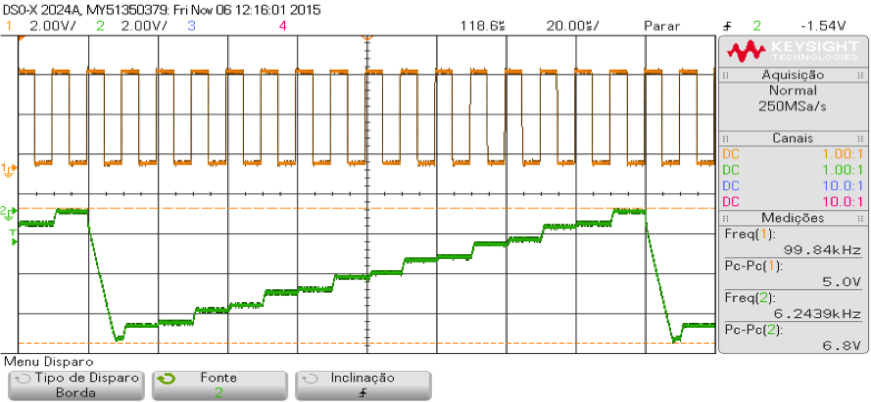
\includegraphics[angle=0,width=0.9\textwidth]{R1_R.png}
     \captionof{figure}{Gráficos $v_o(t)$ (a verde) e $v_{Clk}(t)$ (a laranja) para $R_1=R$, $R_2=R_3=R_4=2R$ e $R_f=4R$, obtidos pelo osciloscópio digital via \textit{Microsoft Excel}.}
     \label{fig:R1_R}
     \end{center}


\begin{center}
     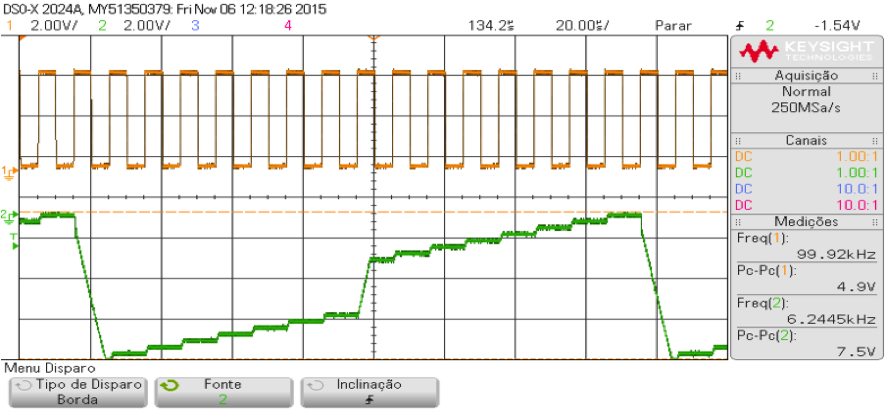
\includegraphics[angle=0,width=0.9\textwidth]{R4_R.png}
     \captionof{figure}{Gráficos $v_o(t)$ (a verde) e $v_{Clk}(t)$ (a laranja) para $R_4=R$, $R_1=R_2=R_3=2R$ e $R_f=4R$, obtidos pelo osciloscópio digital via \textit{Microsoft Excel}.}
     \label{fig:R4_R}
     \end{center}

\subsection{Monoticidade do conversor}

Tal como previsto na análise teórica, ao diminuir a resistência associada a um bit do conversor, o peso deste bit vai aumentar em relação aos outros, o que faz com que a variação de tensão à saída do conversor seja maior quando existe uma alteração de estado desse bit.

Desta forma, verifica-se que ao diminuir o valor de $R_1$ de $2R$ para $R$, o bit $b_1$, a que está associada esta resistência, torna-se o menos significativo, pois no gráfico da figura \ref{fig:R1_R} observamos que ocorre uma maior mudança de tensão a cada dois ciclos de relógio, ou seja, quando à uma transição de $b_1b_2b_3b_4$ de $XXX0$ para $XXX1$.

Já no caso em que se diminui a resistência $R_4$ de $2R$ para $R$, o bit $b_4$, a que está associada esta resistência torna-se o mais significativo, como se pode observar no gráfico da figura \ref{fig:R4_R}, onde se verifica uma maior variação de tensão após 8 ciclos de relógio, do que nas outras transições, que corresponde à passagem de $b_1b_2b_3b_4$ de $0111$ para $1000$.

\chapter{Tempo de estabelecimento}
Pretende-se nesta secção estudar o tempo de estabelecimento do conversor em análise. Para tal, assumir-se-à que este tem origem apenas no tempo de estabelecimento do AMPOP integrado no circuito que, por sua vez, se encontra relacionado com o \emph{slew rate} (SR) do mesmo.\\
O \emph{slew rate} de um amplificador operacional é, por definição, o declive máximo da tensão de saída $v_0$ ou, por outras palavras, a taxa de variação máxima de $v_0$.
\begin{equation}
SR=\left(\dfrac{d\, v_0}{d\, t}\right)_{\textrm{máx}}
\end{equation}

O SR é a característica do amplificador que modela a sua não-idealidade relativamente ao tempo de resposta da entrada para a saída. Num AMPOP ideal, o SR seria infinito e a saída teria variações síncronas com a entrada. Na prática existe sempre um atraso temporal, designado tempo de estabelecimento, o que implica um SR finito.

\section{Análise Teórica}

Para o AMPOP utilizado (741), assumiu-se como valor teórico do SR o valor típico de $0.5\;V/\mu$s. Com este valor, é-nos possível determinar a previsão teórica para o tempo de estabelecimento ($t_s$) do circuito em estudo se conhecermos a variação máxima de tensão que impomos ao conversor.\\

Relembre-se a equação \ref{eq:v02R} que relaciona $v_0$ com a palavra digital para $R_f=2R$:
\begin{equation}
v_0=-\frac{5}{3}\left(\frac{b_1}{8}+\frac{b_2}{4}+\frac{b_3}{2}+b_4\right)\tag{\ref{eq:v02R}}
\end{equation}

Substituindo na equação anterior os coeficientes $b_i$ de forma a obter o valor de $v_0$ para as palavras $b_1b_2b_3b_4=1111$ e $b_1b_2b_3b_4=0000$ é possível, subtraíndo os resultados, determinar a variação máxima de $v_0$, dado que a primeira palavra representa o mínimo de $v_0$ e a segunda o máximo.
\begin{equation}
|\Delta v_0|_{\textrm{máx}}=|v_0(b_1b_2b_3b_4=1111)-v_0(b_1b_2b_3b_4=0000)|=\frac{25}{8}
\end{equation}

Assumindo então que o tempo de estabelecimento do conversor se deve apenas ao \emph{slew rate} do AMPOP, vem:
\begin{equation}
t_{s_{\textrm{teo}}}=\dfrac{|\Delta v_0|_{\textrm{máx}}}{SR_{\textrm{teo}}}=\frac{25}{8}/0.5=6.25\;\mu\textrm{s}
\end{equation}

Dado que a variação da tensão de saída é igual quando se passa de $b_1b_2b_3b_4=1111$ para $b_1b_2b_3b_4=0000$ ou para a transição inversa, conclui-se que o tempo de estabelecimento também será igual.

\section{Análise Experimental}

De forma a estudar o tempo de estabelecimento do conversor, ligou-se o \emph{reset} do contador ao nível lógico ``1'' (5V) e aplicou-se uma onda quadrada de frequência $100$kHz e amplitude 5V no ponto A. Este esquema de montagem permite obter, à entrada do conversor
\begin{equation*}
\left\{ \begin{matrix*}[l]
 S_1S_2S_3S_4=1111 && \textrm{para} && A=0\\[0.3cm]
 S_1S_2S_3S_4=0000 && \textrm{para} && A=1
\end{matrix*} \right.
\end{equation*}

Com $R_f=2R$, obteve-se a resposta apresentada de seguida.


\begin{center}
     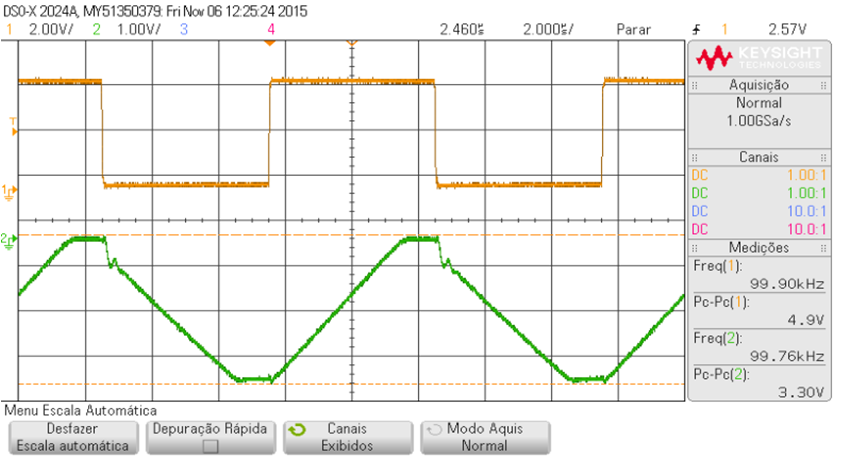
\includegraphics[angle=0,width=0.9\textwidth]{ts2R.png}
     \captionof{figure}{Gráficos $v_o(t)$ (a verde) e $v_{A}(t)$ (a laranja) para $R_f=2R$ obtidos pelo osciloscópio digital via \textit{Microsoft Excel}.}
     \label{fig:ts2R}
     \end{center}

Por observação da figura anterior é possível inferir sobre a importância relativa do estudo do tempo de estabelecimento deste circuito conversor. De facto, observamos que a saída do AMPOP leva quase a totalidade do tempo em que a entrada se encontra num estado para transitar do estado anterior para esse estado actual. Esta resposta diverge muito do que seria um AMPOP ideal com \emph{slew rate} infinito onde a saída acompanharia a entrada sem atrasos no tempo.\\

Tendo em vista a estimação do tempo de estabelecimento experimental, podemos utilizar os três semi-períodos disponíveis na resposta de $v_0$ de forma a ter três estimativas diferentes de $t_s$ para, no fim, assumir como $t_{s_{\textrm{exp}}}$ a média desses três valores. A última transição terá de ser descartada pela razão óbvia de que se encontra truncada antes da estabilização do sinal no nível lógico correcto.\\

A análise dos dados para obtenção do tempo de estabelecimento experimental em cada variação da entrada foi efectuada com o auxílio de software \textit{Matlab} e resume-se aos seguintes passos:
\begin{enumerate}
\item Determinação dos instantes de tempo em que a palavra digital (entrada) muda;
\item Determinação das tensões de saída correspondentes;
\item Determinação dos instantes de tempo em que a saída estabiliza;
\item Determinação das tensões de saída correspondentes;
\item Estimação do tempo de estabelecimento experimental;
\item Estimação do \emph{slew rate} experimental.
\end{enumerate}

O código desenvolvido foi o seguinte.\\

\begin{framed}
\lstset{language=Matlab,%
    %basicstyle=\color{red},
    breaklines=true,%
    morekeywords={matlab2tikz},
    keywordstyle=\color{blue},%
    morekeywords=[2]{1}, keywordstyle=[2]{\color{black}},
    identifierstyle=\color{black},%
    stringstyle=\color{mylilas},
    commentstyle=\color{mygreen},%
    showstringspaces=false,%without this there will be a symbol in the places where there is a space
    numbers=left,%
    numberstyle={\tiny \color{black}},% size of the numbers
    numbersep=9pt, % this defines how far the numbers are from the text
    emph=[1]{for,end,break},emphstyle=[1]\color{red}, %some words to emphasise
    %emph=[2]{word1,word2}, emphstyle=[2]{style},    
}
\lstinputlisting{TempoDeEstabelecimento.m}
\end{framed}

A função integrada TiraRepetidos resume-se a:

\begin{framed}
\lstset{language=Matlab,%
    %basicstyle=\color{red},
    breaklines=true,%
    morekeywords={matlab2tikz},
    keywordstyle=\color{blue},%
    morekeywords=[2]{1}, keywordstyle=[2]{\color{black}},
    identifierstyle=\color{black},%
    stringstyle=\color{mylilas},
    commentstyle=\color{mygreen},%
    showstringspaces=false,%without this there will be a symbol in the places where there is a space
    numbers=left,%
    numberstyle={\tiny \color{black}},% size of the numbers
    numbersep=9pt, % this defines how far the numbers are from the text
    emph=[1]{for,end,break},emphstyle=[1]\color{red}, %some words to emphasise
    %emph=[2]{word1,word2}, emphstyle=[2]{style},    
}
\lstinputlisting{TiraRepetidos.m}
\end{framed}

A execução do código apresentado conduziu então aos resultados organizados na tabela \ref{tab:TsSR}.

\begin{table}[H]
\centering
\begin{tabular}{c|c||c|}
\cline{2-3}                                         & \textbf{Tempo de Estabelecimento $\left[\mu\textrm{s}\right]$} & \textbf{Slew Rate $\left[\textrm{V}/\mu\textrm{s}\right]$} \\ \hline\hline
\multicolumn{1}{||c||}{Valor teórico}      & $6.25$                                                         & $0.5$                                                      \\ \hline
\multicolumn{1}{||c||}{Valor Experimental} & $4.533$                                                        & $0.683$                                                    \\ \hline
\multicolumn{1}{||c||}{Erro relativo}      & $27.467\,\%$                                                   & $36.565\,\%$                                               \\ \hline
\end{tabular}
\caption{Resultados da estimação do tempo de estabelecimento e \emph{slew rate}.}
\label{tab:TsSR}
\end{table}

É possível observar que a variação de tensão de saída máxima experimental (em módulo) é relativamente próxima da prevista teoricamente ($3.125\;\textrm{V}$). De facto, obteve-se:
\begin{equation}
|\Delta v_0|_{\textrm{máx}}=SR_{\textrm{exp}}\times t_{s_{\textrm{exp}}}=3.0955\;\textrm{V}
\end{equation}

Desta forma, dado que a obtenção do tempo de estabelecimento experimental foi efectuada directamente pelas medições, sem cálculos intermédios, podemos concluir que o erro de $\approx 27\%$ advém do facto do valor teórico poder não ser de facto uma boa previsão para o circuito utilizado, ou seja, o valor assumido para o \emph{slew rate} teórico pode de facto não corresponder ao circuito real utilizado no laboratório. Esta conclusão pode ser apoiada por uma análise do valor do erro relativo na medição do tempo de estabelecimento experimental em função do valor teórico considerado para o \emph{slew rate} do AMPOP utilizado. Essa análise resulta no gráfico apresentado de seguida.

\begin{center}
     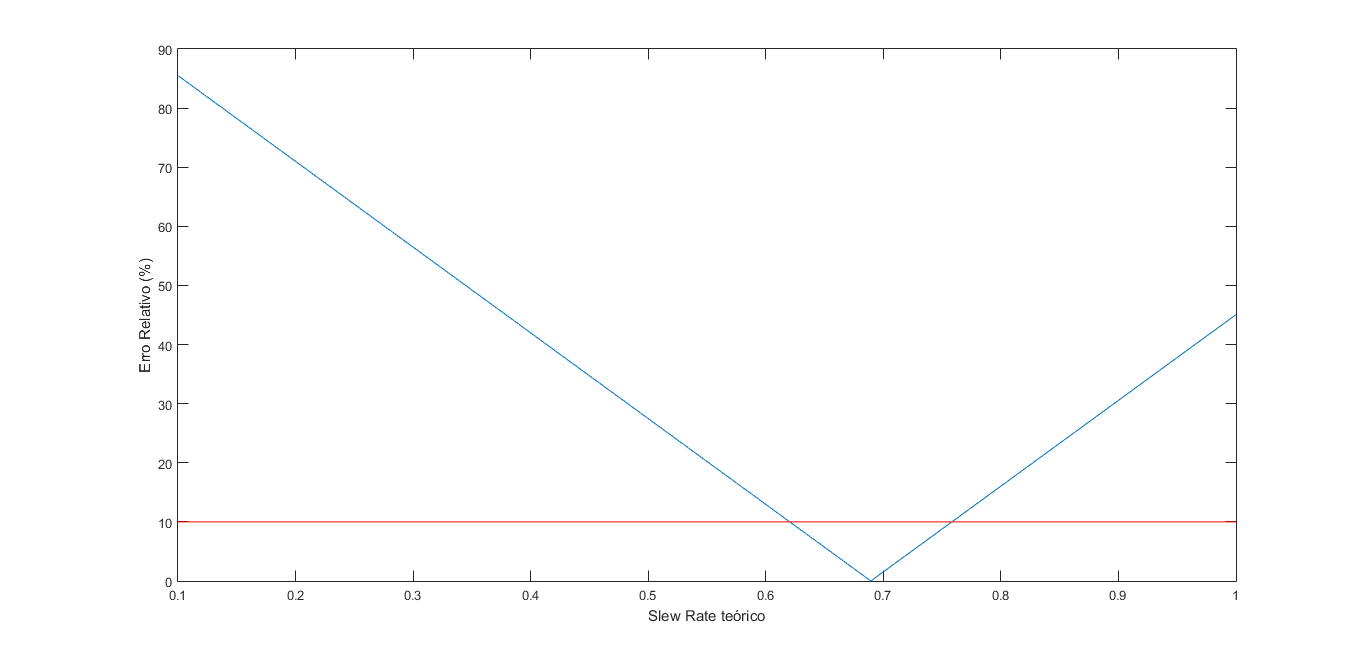
\includegraphics[angle=0,width=1\textwidth]{ErroRelativo6.png}
     \captionof{figure}{Erro relativo da medição de $t_s$ em função do valor de $SR_{\textrm{teo}}$ (a azul) e barreira dos $10\%$ (a vermelho).}
     \label{fig:ErroRelativo6}
     \end{center}
Com esta análise, podemos então concluir que os valores experimentais obtidos, embora apresentem erros relativos próximos de $30\%$, podem ter o seu desvio face ao previsto explicado por uma hipótese inicial incorrecta. Se, devido aos defeitos de fabrico, o \emph{slew rate} verdadeiro do AMPOP fosse de 0.62, o erro relativo obtido experimentalmente seria de apenas $10\%$. Se fosse maior, o erro ainda diminuiria mais até o SR ser maior que 0.689. Assumindo então que o circuito utilizado não possui, pelas condições de fabrico, um \emph{slew rate} de 0.5 mas sim talvez algo mais perto de 0.6 ou 0.7, podemos concluir que o erro experimental de $\approx 37\%$ não advém da qualidade das medições e, portanto, que não nos impede de afirmar que a análise experimental confirma a análise teórica realizada previamente.


\chapter{Picos de tensão na transição de estados}
\section{Sinal de entrada e saída}
Nesta parte do trabalho, a entrada C é mantida a zero (estado \textit{reset}) e é aplicado à entrada A uma onda quadrada de frequência 100kHz e amplitude 5V. Esta onda está representada na figura pela curva a laranja.\par
Com esta montagem, as portas lógicas NOR funcionam como inversores do sinal A (pois a outra entrada da NOR, que vem de C, está sempre a zero), ou seja, quando o sinal A está a high temos uma saída a low e vice versa. No entanto, o bit mais significativo, $S_4$, ainda atravessa a porta lógica NOT que vai inverter novamente o sinal.
Assim, é possível ter dois estados de equílibrio: $S_1S_2S_3S_4 = 1110$ para A=0 e $S_1S_2S_3S_4 = 0001$ para A=1.\par
A saída é representada na imagem pela curva a verde.
\begin{center}
     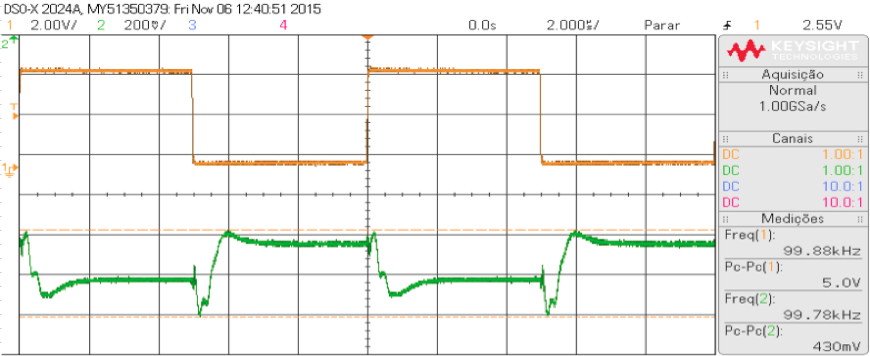
\includegraphics[angle=0,width=1\textwidth]{7_2_1_Sinal_io}
     \captionof{figure}{Sinal de entrada e saida observado}
     \label{7_2_1}
\end{center}

\section{Picos de tensão espúrios}
Os dois patamares estáveis estão situados em $V_0 = -1,63008V$ para o estado $S_1S_2S_3S_4 = 0001$, A=1 e em $V_0 = -1,44893V$ para o estado $S_1S_2S_3S_4 = 1110$, A=0.
Contudo o valor da saída não é sempre estável como se pode constatar na figura seguinte.
\begin{center}
     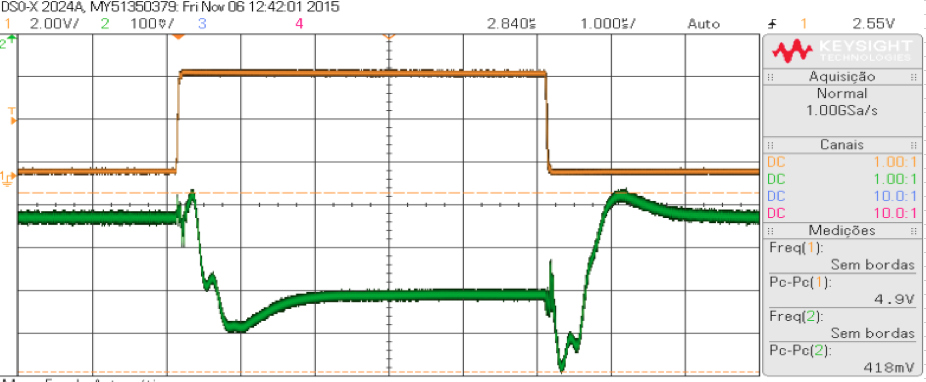
\includegraphics[angle=0,width=1\textwidth]{7_2_2_Atraso}
     \captionof{figure}{Zoom do sinal de entrada e de saída}
     \label{7_2_2}
\end{center}
Nota-se que existe um período oscilatório antes de cada estado estável, existe um \textit{glitch}. Isto é, a tensão de saída que se encontra em -1,63008V (estado 0001) primeiro desce até -1,8002V e depois sobe até -1,3982V e só depois é que estabiliza em -1,44893V (estado 1110). Aquando da transição do estado $1110\rightarrow 0001$ também ocorre o mesmo processo, mas subindo primeiro o valor da tensão e depois descendo, passando o patamar de equilíbrio e voltando a este instantes depois.\par

\section{Análise de Resultados}
Como já foi referido, aquando da transição de estados ocorre um \textit{glitch}, isto é, a tensão de saída não estabiliza instantaneamente. Este efeito pode ser explicado pelo facto de que os componentes do circuito não são ideais, tendo por isso um tempo de \textit{set-up} o que provoca um atraso no tempo. Nomeadamente o efeito da porta NOT (inversor) relativamente ao bit mais significativo $S_4$.\par 
Todos os bits atravessam a porta NOR e o ampop, no entanto, o bit $S_4$ atravessa ainda a porta NOT, atrasando o estado final e gerando um estado quase instantâneo devido ao seu atraso. Este atraso pode ser visto como:
\begin{equation*}
\left\{ \begin{matrix*}[l]
 1110 \rightarrow 1001 \rightarrow 0001\\
 0001 \rightarrow 0110 \rightarrow 1110
\end{matrix*} \right.
\end{equation*}
Posto isto, é possível explicar a intensidade do glitch, pois trata-se do bit com maior peso relativo no valor da tensão de saída e o sistema tende inicialmente a evoluir para um patamar de equílibrio instantâneo que é logo alterado para o patamar de equílibrio efetivo.
\chapter{Conclusões}

Com esta atividade laboratorial houve oportunidade de aplicar conhecimentos adquiridos nas aulas teóricas e presenciar um conversor D/A, implementado pelos alunos, em funcionamento. A utilização do circuito R-2R revela ser uma forma muito fácil e intuitiva de converter sinais digitais em sinais analógicos e ainda bastante versátil para alterar o peso relativo de cada bit se assim for desejado.\par
O conversor digital-analógico permitiu-nos associar a cada palavra digital uma tensão de conversão de valor específico e bem definido. As transições entre palavras consecutivas correspondem a transições uniformes no valor de tensão do sinal analógico. \par Podemos assim concluir que uma boa conversão de sinal, implica um gráfico de sinal analógico regular, com perturbações reduzidas promovendo a injectividade na conversão. \par É ainda importante referir que os valores de tensão dos patamares do gráfico de sinal analógico são múltiplos inteiros do patamar-unidade associado à palavra digital $0001$, sendo a palavra $0000$ associada ao zero de tensão.\par
Adicionalmente, devido às não-idealidades dos componentes do circuito é possível observar pequenos desvios dos resultados teóricos, como seria de esperar de um trabalho experimental. Não existem transições instantâneas e existe um período de resposta que é condicionado pelo \textit{slew rate} do AMPOP. O \textit{slew rate} do AMPOP utilizado é inevitavelmente limitado pelas pequenas correntes internas que o percorrem e também pelas capacitâncias internas desenhadas para compensar oscilações a altas frequências. Embora alguns amplificadores operacionais sejam compensados externamente e, dessa forma, ofereçam algum controlo sobre o \textit{slew rate}, esse não é o caso do AMPOP utilizado.\par
Desta forma, haverá uma frequência máxima à qual o amplificador conseguirá variar a sua tensão de saída. Como a onda quadrada apresenta um espectro de potência com largura de banda infinita, espera-se que a saída do AMPOP não consiga replicar esse sinal no tempo e esteja limitado a uma frequência máxima. Essa característica é modelada pelo \textit{slew rate}, definido então como a taxa máxima de variação da saída do AMPOP.\par
Para o AMPOP utilizado, assumiu-se o valor do \textit{datasheet} de 0.5 V/$\mu$s. Contudo, mesmo admitindo algum ruído experimental, o trabalho laboratorial permitiu concluir que esse valor teórico pode de facto não ser adequado. O motivo aparentemente mais óbvio para o desvio será o de haver defeitos no fabrico que permitam que o valor real obtido para o \textit{slew rate} do AMPOP oscile consideravelmente em torno do valor de projecto. Alternativamente, o uso repetitivo do circuito em laboratório pode, com o tempo, desgastar as componentes internas do AMPOP e promover um maior número de não-idealidades que resultem numa oscilação ainda maior face ao valor projectado.

\end{document}



